% !TEX program = tectonic
\documentclass[12pt,a4paper,oneside,openany]{book}
\usepackage[T1]{fontenc}
\usepackage[utf8]{inputenc}
\usepackage{lmodern}
\usepackage[a4paper,margin=25mm,footskip=12mm]{geometry}
\usepackage{setspace,microtype,graphicx,xcolor,booktabs,longtable,tabularx,array,caption,placeins,amsmath,pdflscape,multirow,amssymb}
\usepackage{xurl}
\usepackage[hidelinks,unicode,pdfencoding=auto]{hyperref}
\hypersetup{pdftitle={Collaborative Tangram in Shared Overhead VR: Shape Judgment and the Coordination of Construction},pdfauthor={Yiyang Qin},pdfsubject={REIT7841 v1.1},pdfkeywords={collaborative VR, Tangram, shared overhead view, shape judgment}}
\onehalfspacing
\setlength{\parindent}{0pt}
\setlength{\parskip}{4pt plus 1pt minus 1pt}
\setlength{\emergencystretch}{2em}
\setcounter{tocdepth}{2}
\setcounter{secnumdepth}{2}
\captionsetup{hypcap=false,font={small,stretch=1.05},labelfont=bf,justification=justified,singlelinecheck=false}
\captionsetup[table]{position=top}
\setlength{\LTcapwidth}{\textwidth}
\renewcommand{\topfraction}{0.88}
\renewcommand{\bottomfraction}{0.8}
\renewcommand{\textfraction}{0.12}
\renewcommand{\floatpagefraction}{0.7}
\widowpenalty=10000
\clubpenalty=10000
\displaywidowpenalty=10000
\raggedbottom
\pagestyle{plain}

% Keep each figure with its local explanation at a paragraph boundary.
\newsavebox{\figureunitbox}
\newenvironment{figureunit}[1]{%
  \def\figureunitid{#1}%
  \par\addvspace{8pt}\noindent
  \begin{lrbox}{\figureunitbox}\begin{minipage}{\linewidth}%
  \setlength{\parskip}{4pt plus 1pt minus 1pt}%
}{%
  \end{minipage}\end{lrbox}%
  \typeout{LAYOUTUNIT \figureunitid: \the\dimexpr\ht\figureunitbox+\dp\figureunitbox\relax}%
  \usebox{\figureunitbox}\par\addvspace{8pt}%
}
\brokenpenalty=10000

\begin{document}
\frontmatter
% v1.1 AI statement. Preserve the 12-column form from ThesisPlan PDF p.6.
% Requires pdflscape, longtable, array, graphicx, multirow, amssymb and setspace.
\chapter*{Use of AI Statement}
\addcontentsline{toc}{chapter}{Use of AI Statement}
\noindent\textbf{v1.1}

I acknowledge the use of AI tools in this project. The table records their use from the first-semester proposal through the present thesis. I take responsibility for evaluating and integrating the assisted material and for the final submitted work.

I conducted the study and formed its findings and key observations. I supplied the behavioural accounts, selected the important cases, and corrected their interpretation. AI assisted with checking those accounts against selected source records, organising the material, computing and drawing selected representations, and expressing the work in English. It also supported earlier planning, literature reading, Unity prototype coding and debugging, research-logging implementation, and document preparation.

The original Thesis Plan table structure is retained below. A tick identifies a documented use in that stage. ``Data analysis'' includes assisted data organisation, numerical checks and selected log or geometric verification; it does not attribute the discovery of the findings to AI. ``Visual content creation'' includes document formatting and programmatic figures made from recorded data. No participant observations or questionnaire answers were generated by AI. Software coding, debugging and data-capture implementation are described under ``Other use'' because the original form has no separate code column. Tool names are reported where exact model versions were not retained. Semester-level dates are used where the early records do not establish a reliable usage day.

\begin{landscape}
\begingroup
\setstretch{1}
\fontsize{10}{12}\selectfont
\setlength{\tabcolsep}{2pt}
\renewcommand{\arraystretch}{1.1}
\setlength{\LTpre}{0pt}
\setlength{\LTpost}{0pt}
\begin{longtable}{|>{\raggedright\arraybackslash}p{0.14\linewidth}|*{10}{>{\centering\arraybackslash}p{0.027\linewidth}|}>{\raggedright\arraybackslash}p{\dimexpr0.59\linewidth-24\tabcolsep-13\arrayrulewidth\relax}|}
\hline
\multirow{2}{*}{\shortstack{\textbf{AI model}\\\textbf{and date}}} & \multicolumn{11}{c|}{\textbf{Artificial Intelligence (AI) tool usage} (tick all that apply)} \\
\cline{2-12}
 & \rotatebox{90}{\strut Topic exploration} & \rotatebox{90}{\strut Research question} & \rotatebox{90}{\strut Literature review} & \rotatebox{90}{\strut Methodological support} & \rotatebox{90}{\strut Data analysis} & \rotatebox{90}{\strut Visual content creation} & \rotatebox{90}{\strut Written content creation} & \rotatebox{90}{\strut Language translation} & \rotatebox{90}{\strut Grammar/style/spelling} & \rotatebox{90}{\strut Feedback on content} & \multicolumn{1}{c|}{\shortstack{Other use\\(provide details)}} \\
\hline
\endfirsthead
\hline
\multirow{2}{*}{\shortstack{\textbf{AI model}\\\textbf{and date}}} & \multicolumn{11}{c|}{\textbf{Artificial Intelligence (AI) tool usage} (tick all that apply)} \\
\cline{2-12}
 & \rotatebox{90}{\strut Topic exploration} & \rotatebox{90}{\strut Research question} & \rotatebox{90}{\strut Literature review} & \rotatebox{90}{\strut Methodological support} & \rotatebox{90}{\strut Data analysis} & \rotatebox{90}{\strut Visual content creation} & \rotatebox{90}{\strut Written content creation} & \rotatebox{90}{\strut Language translation} & \rotatebox{90}{\strut Grammar/style/spelling} & \rotatebox{90}{\strut Feedback on content} & \multicolumn{1}{c|}{\shortstack{Other use\\(provide details)}} \\
\hline
\endhead
\hline
\multicolumn{12}{r}{\textit{Continued on the next page}}\\
\endfoot
\hline
\endlastfoot
\textbf{ChatGPT}\newline Semester 1, 2026 & \ensuremath{\checkmark} & \ensuremath{\checkmark} &  & \ensuremath{\checkmark} &  &  & \ensuremath{\checkmark} & \ensuremath{\checkmark} & \ensuremath{\checkmark} & \ensuremath{\checkmark} & \textbf{Topic definition and early study planning.} Helped organise the author's ideas, discuss possible research framings and study structures, and turn early planning notes into clearer text. The author and supervisor made the research decisions. \\
\hline
\textbf{ChatGPT}\newline Semester 1, 2026 &  &  & \ensuremath{\checkmark} &  &  &  & \ensuremath{\checkmark} & \ensuremath{\checkmark} & \ensuremath{\checkmark} & \ensuremath{\checkmark} & \textbf{Literature reading and proposal writing.} Explained difficult passages, compared the relevance of papers located by the author, and assisted with proposal organisation, Chinese-to-English translation and wording. Literature claims remained tied to the cited sources. \\
\hline
\textbf{Gemini Pro}\newline Semester 1, 2026 &  &  &  &  &  & \ensuremath{\checkmark} & \ensuremath{\checkmark} & \ensuremath{\checkmark} & \ensuremath{\checkmark} &  & \textbf{Proposal typesetting.} Assisted with translation, language correction, visual formatting and LaTeX code for the proposal, as disclosed in that document. Visual content creation here refers to document formatting. \\
\hline
\textbf{ChatGPT}\newline Semester 1, 2026 &  &  &  & \ensuremath{\checkmark} &  &  & \ensuremath{\checkmark} & \ensuremath{\checkmark} & \ensuremath{\checkmark} & \ensuremath{\checkmark} & \textbf{Ethics wording and meeting notes.} Assisted with wording for draft ethics and study-planning documents, and with organising supervisor-meeting notes and follow-up tasks. \\
\hline
\textbf{ChatGPT / OpenAI Codex}\newline 17--19 August 2026 & \ensuremath{\checkmark} & \ensuremath{\checkmark} & \ensuremath{\checkmark} & \ensuremath{\checkmark} &  &  & \ensuremath{\checkmark} & \ensuremath{\checkmark} & \ensuremath{\checkmark} & \ensuremath{\checkmark} & \textbf{Thesis Plan.} Reorganised existing proposal and project material for the Thesis Plan, compared research framings, drafted connecting English text, and prepared LaTeX formatting. \\
\hline
\textbf{OpenAI Codex}\newline September 2026 &  & \ensuremath{\checkmark} &  & \ensuremath{\checkmark} &  &  & \ensuremath{\checkmark} & \ensuremath{\checkmark} & \ensuremath{\checkmark} & \ensuremath{\checkmark} & \textbf{Method and prototype preparation.} Reviewed the author's plans and supervisor feedback, helped refine questionnaire and interview procedures, and organised prototype, viewing-orientation and recording requirements. The author supplied revisions and selected the implemented procedure. \\
\hline
\textbf{OpenAI Codex}\newline 20--23 September 2026 &  &  &  & \ensuremath{\checkmark} &  &  & \ensuremath{\checkmark} &  &  &  & \textbf{Multiplayer prototype coding and debugging.} Wrote and revised Unity C\# scripts and scene configuration for the two-player prototype, object synchronisation, grab/release control, first-person and overhead display, connection menus and builds. Debugging followed the author's headset-test feedback; technical instructions were also prepared. \\
\hline
\textbf{OpenAI Codex}\newline 6--7 October 2026 &  &  &  & \ensuremath{\checkmark} &  &  & \ensuremath{\checkmark} &  &  &  & \textbf{Research logging implementation.} Implemented and checked the ResearchV2 CSV logger and its connections to piece actions, recorded poses, round controls and participant/round identifiers. Prepared validation code, builds and export guidance. \\
\hline
\textbf{OpenAI Codex}\newline 6--7 October 2026 &  &  &  & \ensuremath{\checkmark} &  &  & \ensuremath{\checkmark} & \ensuremath{\checkmark} & \ensuremath{\checkmark} & \ensuremath{\checkmark} & \textbf{Collection materials.} Revised the Chinese collection guide, moderator manual, researcher record sheet and twelve-item questionnaire; documented Unity log fields and later evidence use. \\
\hline
\textbf{OpenAI Codex}\newline 7--10 October 2026 &  &  &  & \ensuremath{\checkmark} &  &  & \ensuremath{\checkmark} &  &  &  & \textbf{Prototype revisions and technical checks.} Implemented the shared target, manual round ending and overhead-menu repair, then target grabbing, ray interaction and the later view adjustment. Produced checks and APK builds from the author's requirements and reported faults. Each revision retained its version identity. \\
\hline
\textbf{ChatGPT / OpenAI Codex}\newline 13--14 October 2026 &  &  & \ensuremath{\checkmark} &  & \ensuremath{\checkmark} &  & \ensuremath{\checkmark} & \ensuremath{\checkmark} & \ensuremath{\checkmark} & \ensuremath{\checkmark} & \textbf{Conference paper.} Organised researcher-provided case records and questionnaire summaries, supported comparison of evidence across sources, and helped draft, translate, edit and format the conference paper. The author supplied observations and participant responses. \\
\hline
\textbf{ChatGPT / OpenAI Codex}\newline 16--21 October 2026 &  &  &  & \ensuremath{\checkmark} & \ensuremath{\checkmark} & \ensuremath{\checkmark} & \ensuremath{\checkmark} &  & \ensuremath{\checkmark} & \ensuremath{\checkmark} & \textbf{Corpus organisation and data reconciliation.} Indexed videos, reports, interviews and logs; organised the author's observations; checked selected records; reconciled the 48 confirmed questionnaire responses; and produced descriptive tables, evidence maps and programmatic plots. \\
\hline
\textbf{TurboScribe}\newline Records retrieved 20 October 2026 &  &  &  &  &  &  &  &  &  &  & \textbf{Meeting transcription.} Automatic transcription of recorded supervisor meetings used to recover project history. Existing text and subtitle exports were retrieved on 20 October; this is an archive date, not a claimed transcription date for every recording. \\
\hline
\textbf{ChatGPT / OpenAI Codex}\newline 21--22 October 2026 &  &  & \ensuremath{\checkmark} &  & \ensuremath{\checkmark} & \ensuremath{\checkmark} & \ensuremath{\checkmark} & \ensuremath{\checkmark} & \ensuremath{\checkmark} & \ensuremath{\checkmark} & \textbf{Poster and presentation.} Checked selected action sequences and reconstructed geometry for the author's observations; prepared programmatic figures, poster text and layout; and revised speaking notes from the author's oral explanations. The author chose the findings and corrected the accounts. \\
\hline
\textbf{ChatGPT / OpenAI Codex}\newline 25 October--2 November 2026 &  &  & \ensuremath{\checkmark} & \ensuremath{\checkmark} & \ensuremath{\checkmark} & \ensuremath{\checkmark} & \ensuremath{\checkmark} & \ensuremath{\checkmark} & \ensuremath{\checkmark} & \ensuremath{\checkmark} & \textbf{Thesis integration and revision.} Organised thesis sources and sections; checked selected logs, geometry and references; produced code-based figures; drafted and revised English from the author's material; and prepared LaTeX, tables, this disclosure and PDF checks. \\
\hline
\end{longtable}
\endgroup
\end{landscape}

\clearpage
\chapter*{Abstract}
\addcontentsline{toc}{chapter}{Abstract}

A shared overhead view gives collaborators access to the same spatial arrangement while they act on a developing construction. This thesis examines how that view relates to shape judgment and the coordination of work in collaborative Tangram solving. Six pairs took part in four conditions: physical direct viewing, physical overhead video, first-person VR and shared overhead VR. The analysis follows their construction processes through the researcher's observations, video recordings, selected action and pose logs, questionnaires and interviews.

Three connected findings emerged. First, near-complete constructions in first-person VR could look convincing while leaving a piece unused or differing from the target outline. The same class of problem was not observed in the shared-overhead VR records, where the planar relationships were directly visible. Second, participants expressed ideas by placing pieces, and their partners could continue those placements or demonstrate an alternative. The division of work changed during a task as people moved between separate attempts, assistance and joint reconstruction. Third, several episodes showed a partner retaining or extending a local construction that its original builder later revised, including cases where a correct part was lost. Other episodes showed direct partner intervention when an alternative was put into action.

These findings connect the geometric advantage of an overhead view with the actions through which partners develop and judge a shared solution. They support combining an inspectable overview with usable manipulation, brief assistance and access to earlier constructions during revision.

\vspace{0.6em}
\noindent\textbf{Keywords:} collaborative virtual reality; shared overhead view; Tangram; shape judgment; action coordination

\clearpage
\tableofcontents
\clearpage
\listoffigures
\clearpage
\listoftables

\mainmatter
\chapter{Introduction}\label{chap:1}

Solving a Tangram together involves continually relating a small placement to a developing whole. One participant may try a triangle as a head while the other works on the body. A promising arrangement can guide the next move, expose a disagreement or be dismantled when the remaining pieces do not fit. The partners must judge the shape they are building while deciding how to respond to each other's actions. The view of the workspace is therefore part of the practical organisation of the task.

Shared visual information can help people follow task progress and establish what a partner means \cite{gutwin2002,gergle2013}. In virtual reality (VR), designers can change both the viewpoint and the way a participant reaches and manipulates objects. A first-person view places the user within the scene. An external view can expose the arrangement from outside it. For a planar puzzle, a perpendicular overhead view also provides a direct view of the outline and the relations between pieces. These properties make shared overhead viewing a useful setting for examining how visual access and collaborative action work together.

The project began with a supervisor-defined brief about collaborative behaviour in third-person VR. Its focus was how participants communicate intentions, coordinate actions and positions, negotiate object manipulation and maintain awareness of a shared workspace. Physical activity and conventional first-person VR provided comparison contexts. The implemented prototype develops this brief through a shared overhead view and a common Tangram task family. Both participants can manipulate pieces and decide how to divide or combine their work.

A shared view makes an arrangement available to inspect, but the pair still has to decide what to do with it. A participant can demonstrate an idea through a placement, continue a partner's partial solution or challenge it by trying another configuration. What remains on the table also matters: an earlier construction can become the starting point for later work. Following these sequences connects the display to the participants' use of it, including the moments when they keep a useful part, reopen it or accept a shape that does not match the target.

The research asks how this process develops in shared overhead VR and how comparison with other viewing conditions helps explain it. The overall research question is: How do pairs use shared overhead VR to judge and develop a Tangram construction together, and how do these processes relate to those observed in physical viewing and first-person VR?

RQ1: What shape-judgment problems arise during construction in the implemented viewing conditions, and how do participants check and respond to them?

RQ2: How do participants express local ideas through speech and manipulation, continue one another's work and reorganise who performs an action?

RQ3: How are partial constructions retained, extended or revised by their original builder and by the partner as the joint task develops?

Six pairs took part in physical direct viewing, physical overhead video, first-person VR and shared-overhead VR, in that order. The study uses researcher-prepared process records, group interviews, post-round questionnaires and available system records. The central analysis follows selected interaction sequences and reconstructs relevant VR arrangements from recorded piece poses. Action logs identify who controlled a piece and when; process records supply the surrounding proposal, response and task context. Together they make changes in both participation and geometry inspectable.

The findings bring three aspects of the task into one account. First-person VR included plausible constructions with unused pieces or incorrect proportions. G06's accepted candle provides a particularly clear example: incorporating all seven pieces resolved one visible problem while leaving a proportion mismatch. The pair's changing work on that construction also shows how initially separate local activity became shared reconstruction. Other cases show partners retaining or extending an arrangement that its original builder later changed, sometimes removing a correct partial solution.

The thesis contributes an empirical account of shared overhead VR within a broader set of collaborative viewing arrangements. Its contribution lies in connecting geometric judgment to the sequence of proposals, placements, continuations and revisions through which the pair produces a result. The fixed condition order, task patterns and prototype versions define the comparison and are considered in the method and discussion. Design implications concern access to the overall shape, usable manipulation, brief assistance and the preservation of earlier work during exploration.

Chapter~\ref{chap:2} establishes the concepts used to examine visible activity and collaborative problem solving. Chapters 3 and 4 describe the project's development, prototype and study method. Chapters 5 and 6 present the findings and discuss their implications for shared overhead VR. Chapter~\ref{chap:7} concludes the thesis.


\chapter{Related Research and Analytic Concepts}\label{chap:2}

Shared-view interfaces change both the information available to collaborators and the ways they can act on it. This chapter connects research on visual access with accounts of how people develop and revise a shared task. The comparison centres on three questions: what a view makes inspectable, how a partner's actions become usable, and how contributions remain connected as control changes.

\section{Seeing the workspace and understanding a contribution}\label{sec:2-1}

A common image gives partners access to a task state, while their responses establish what they understand about it. Clark and Brennan describe grounding as establishing that a contribution has been understood sufficiently for the current purpose \cite{clark1991}. Gergle, Kraut and Fussell distinguish this work from maintaining awareness of the current situation; their experiments examine visual immediacy, perspective alignment and common viewing area \cite{gergle2013}. The distinction is useful in construction tasks. Seeing where a piece has been placed, understanding the proposed relation and accepting the whole arrangement as correct are separate achievements.

The shared state also changes as people work. Roschelle and Teasley's joint problem space connects goals, descriptions of the problem and available actions through the partners' ongoing activity \cite{roschelle1995}. Gutwin and Greenberg explain how bodies, communication and the visible effects of manipulation provide workspace awareness. Their concept of feedthrough identifies the information that object changes make available to others \cite{gutwin2002}. Read together, these accounts connect a placement to the partner's next response. An arrangement can communicate an idea, provide a reference for another move or become the part that the pair later reconsiders.

Recent studies make the changing demand for this information visible. In six VR--desktop pairs, Saffo et al. found that sharing interactions and perspectives helped partners follow one another when moving towards closer collaboration \cite{saffo2023}. Irlitti et al.'s six three-person groups in hybrid workspaces showed that one person's manipulation could accompany either active discussion by others or relatively disengaged watching \cite{irlitti2024}. Both studies connect participation to the surrounding activity. For Tangram, this supports examining what a move responds to and what it enables next, alongside who holds the piece.

\section{What different shared views support}\label{sec:2-2}

Shared perspective is implemented through several distinct mechanisms. TeamPortal provides an interactive parallel view into a partner's field of view \cite{wang2025}. MAGIC transforms the partner's representation so that gestures remain meaningful across spatial arrangements while retaining face-to-face interaction \cite{fidalgo2023}. SPARC combines a common orientation with transformed avatar arms and references; its evaluation uses assigned assembler and instructor roles in three-dimensional assembly \cite{simoes2025}. These systems respectively emphasise access to another view, alignment of embodied references and persistent shared orientation. They show why camera position, partner representation and control mapping need separate description when comparing interfaces.

The value of an overview depends on the spatial demands of the task. Chen et al. compared a world-in-miniature, an interactive 2D map and a static terrain map with 18 pairs. Interactive views improved performance over the baseline, and the miniature was more useful in complex scenes involving occlusion \cite{chen2024}. Chang, Lee and Yoo compared 2D video, a 360-degree view and a reconstructed 3D view in VR--AR assistance. Thirty participants each worked with an actor; the independently explorable 3D view supported faster guidance, while the 360-degree view was preferred for the feeling of being together \cite{chang2024}. Both comparisons link richer access to spatial information with particular task benefits, while Chang et al. also separate those benefits from social experience.

These comparisons involve different forms of control and cooperation. Chen et al.'s map supports horizontal movement, whereas the miniature supports three-dimensional operations. Chang et al.'s task assigns expert and worker roles. In a constrained passenger-space assembly task, Medeiros et al. instead varied the users' spatial arrangement. Side-by-side placement was preferred for visibility and object control, and face-to-face placement offered stronger social presence; completion time and correct-piece counts did not differ significantly \cite{medeiros2024}. A favourable experience of the view therefore needs to be related to the action and outcome it supports.

Communication frequency requires similar interpretation. Basille, Lavou\'e and Serna's desktop serious-game study with six triads associated first-person viewing with more information sharing, which the authors related to differences in what players could see \cite{basille2022}. This provides a useful comparison with shared-overview designs: additional communication can supply information missing from a participant's view. Its frequency alone says little about whether the pair can judge the developing configuration accurately.

Tangram makes precise planar relationships central to this comparison. Chen et al. identify overlap in a 2D projection as a problem, and their placement task leaves finer placement accuracy for further investigation \cite{chen2024}. In Tangram, relative widths, orientations and edges determine whether a candidate matches the target. A perpendicular orthographic view preserves these planar relations without perspective depth scaling. The present study examines how partners use the available view while forming, inspecting and accepting a construction, bringing geometric judgment into the analysis of collaborative action.

\section{Connecting visual access with control}\label{sec:2-3}

Partners can understand the same construction while having different practical access to its pieces. Irlitti et al.'s physical, volumetric and virtual objects offered different possibilities for direct action \cite{irlitti2024}. Medeiros et al.'s spatial formations also changed visibility and object control \cite{medeiros2024}. These studies connect the organisation of participation to the way the interface distributes action. This is relevant to the present overhead prototype, where the shared camera image and the tracked movement of each controller use different frames of reference. A clearly visible next step may still be difficult for one partner to execute.

Making the current action state visible can help coordinate that execution. In a screen-based virtual environment with hand tracking, Kim and Park examined feedback about the user's and partner's states during joint movement and handover \cite{kim2024}. Their study addresses the timing of coordinated manipulation. Combined with the changing awareness needs found by Saffo et al. \cite{saffo2023}, it suggests examining assistance as an episode: one participant encounters a difficulty, a partner gains enough information to act, and control or responsibility changes for the next step. The relevant question is how that transfer advances the shared construction.

\section{Developing ideas through temporary divisions of work}\label{sec:2-4}

Manipulation can help develop a proposal as well as communicate it. Hornecker and Buur connect lightweight, legible manipulation with the social organisation of tangible interaction \cite{hornecker2006}. Kirsh and Maglio's analysis of Tetris explains how moving or rotating a piece can make a spatial problem easier to assess \cite{kirsh1994}. Their accounts give complementary reasons to examine tentative placements: the action can help its maker work out a relation and make that relation available to a partner. Kirsh and Maglio also recognise that the same move may advance the task and help determine what to do. Its role is interpreted through the surrounding sequence.

The resulting division of work can be brief. Dillenbourg discusses cooperation and collaboration in terms of the grain and organisation of activity, including spontaneous division and changing, intertwined roles \cite{dillenbourg1999}. Gutwin and Greenberg similarly address movement between independent activity and closer joint work \cite{gutwin2002}. These accounts accommodate a pair that develops different parts for a time and then returns to a common difficulty. The connection between contributions lies in how one person's work extends, adjusts or replaces what the other has made.

Measurement needs to preserve this distinction. In Yang et al.'s VR--desktop image-organisation study, 40 participants worked in groups of four. VR groups showed more conversation and object interaction, with more equal contributions to grabbing, while speed and accuracy were similar \cite{yang2022}. Their measures distinguish picking up an image from regrouping it. Irlitti et al.'s distinction between engaged discussion and watching further shows why a count of direct operations needs contextual interpretation \cite{irlitti2024}. For Tangram, an accepted grab identifies control; the resulting configuration and the partner's response establish whether it was a small adjustment, a new proposal or a structural revision.

\section{Keeping and revising a partner's work}\label{sec:2-5}

A construction remains available after its builder releases it. Preserving, extending and replacing that arrangement have different consequences for the shared task. Yang et al. examined requests for permission before changing another person's image grouping \cite{yang2022}. Rasch et al. studied undo with 16 pairs building towers in VR: world undo increased reported connectedness while also creating opportunities to interfere with a partner's work \cite{rasch2024}. Together, these studies make both the surrounding exchange and the extent of a change relevant. Retained geometry establishes that earlier work remains available; talk or retrospective accounts can explain what that retention means to the participants.

Rasch et al. also identify changing collaboration arrangements as an issue beyond their deliberately divided and collaborative task settings \cite{rasch2024}. Dillenbourg's account of intertwined work helps connect this issue to short construction episodes \cite{dillenbourg1999}. One person may build a part, another may continue it, and the original builder may later reopen it. A local alternative can redirect the next step before either partner has a complete solution. Following who formed and changed the arrangement makes those developments visible.

This thesis connects these questions through the evolving Tangram configuration. Viewpoint research establishes why task geometry, orientation and control matter. Grounding and workspace awareness explain why the response to a placement matters. Research on manipulation, division of work and revision provides concepts for examining how partial contributions persist and change. The study follows these relationships across physical and VR conditions to identify what shared-overhead VR needs to support.

\chapter{Research development and prototype}\label{chap:3}

\section{From the original brief to a shared task family}\label{sec:3-1}

The project began with a familiar physical construction task as a basis for investigating collaboration in VR. Early planning used Tangram to examine communication, coordination and awareness before moving into a virtual environment. The first physical test plan recorded prospective sample ranges, timing and ordering arrangements. The final study procedure is described in Chapter~\ref{chap:4}. [\hyperlink{src:D28}{D28}, \hyperlink{src:D29}{D29}, \hyperlink{src:D30}{D30}]

During the first semester, supervisor discussions encouraged an explicit research aim alongside the technical prototype. The June discussion considered how participants might work on separate parts or jointly take responsibility for a task. This kept the project open to different forms of cooperation rather than requiring both people to touch the same object. It also established why observing the organisation of work would be relevant to a viewpoint study. [\hyperlink{src:D34}{D34}, \hyperlink{src:D35}{D35}]

The early expectations concerned both spatial understanding and the organisation of work. In an email of 19 August, the researcher proposed that a shared external view might make the overall workspace and the partner's activity easier to understand, while making individual working areas and agency less clearly separated. First-person viewing was expected to allow clearer personal areas or divisions of work. These possibilities guided what to observe as the project developed. The study retained the exploratory aim discussed with the supervisor: to understand differences in collaborative activity through a working prototype. [\hyperlink{src:D32}{D32}, \hyperlink{src:D34}{D34}, \hyperlink{src:D31}{D31}]

The August plan developed the idea of shared spatial representations. It considered physical Tangram, VR Tangram for familiarisation and a more open VR construction task, such as building a vehicle. The accompanying email recognised that spatial overlap or activity alone would be insufficient as a measure of collaboration quality. The present analysis follows that concern by examining the sequence and meaning of actions rather than their volume. [\hyperlink{src:D31}{D31}, \hyperlink{src:D32}{D32}]

The supervisor's response on 20 August explained why using a common task family would strengthen comparison. Changing from physical Tangram to an entirely different VR activity would introduce task differences alongside the intended viewpoint comparison. The 1 September meeting revisited the alternatives of using construction blocks in every condition or Tangram in every condition. Tangram was selected to focus the implementation on the original collaboration question. [\hyperlink{src:D33}{D33}, \hyperlink{src:D36}{D36}]

\begin{figureunit}{3-1}
The same feedback questioned the assumption that a collaborative task must be indivisible. Participants can work on separate parts and still choose when to work together. An intermediate test table contained eight combinations, including prescribed roles and free collaboration. After trying the procedure, the researcher removed prescribed roles because they made the testing more complicated and restricted how partners organised the task. The final design let both participants manipulate pieces and negotiate their own next actions. This made temporary division, assistance and changes of initiative available for observation. [\hyperlink{src:D37}{D37}, \hyperlink{src:D69}{D69}, \hyperlink{src:D38}{D38}]

\par\begingroup
\centering
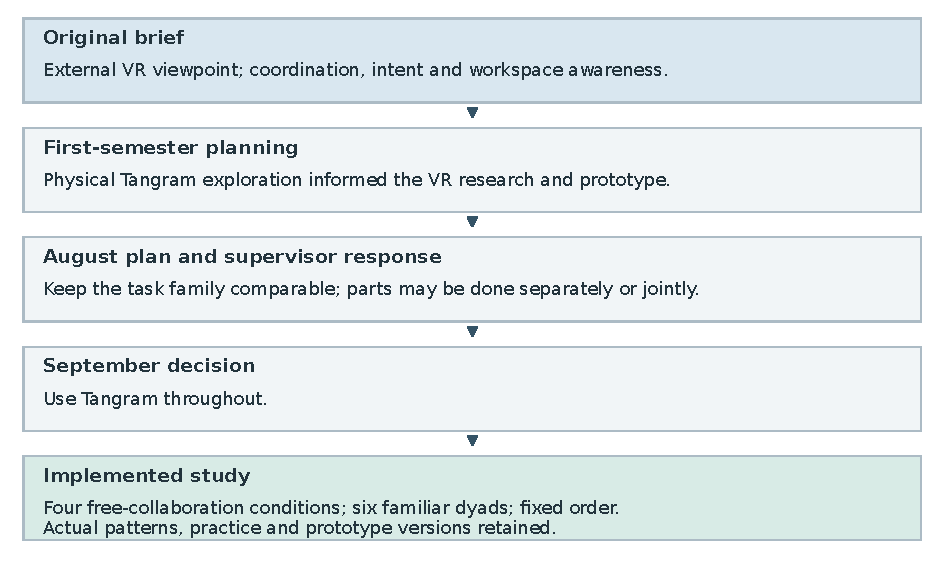
\includegraphics[width=\linewidth,height=95mm,keepaspectratio]{assets/figures/Figure3_1_research_development.pdf}
\captionof{figure}[Development of the research focus and study design.]{Development of the research focus and study design. The August feedback called for a comparable task family while retaining the possibility of individual and joint work. The September discussion selected Tangram across the tasks. The final four-condition study is shown separately from those earlier plans. Sources: original project brief, early study plan, August thesis plan and supervisor response, 1 September meeting transcript, and final study procedure.}\label{fig:3-1}
\par\endgroup
\end{figureunit}




\section{The physical and virtual arrangements}\label{sec:3-2}

\begin{figureunit}{3-2}
The four conditions changed the visual access to a shared Tangram workspace while retaining a common construction task. Figure~\ref{fig:3-2} shows the physical apparatus and the virtual display arrangements. In each condition both partners could manipulate pieces and propose placements. The arrangements are described separately because a shared image and an intuitive mapping from hand movement to that image are different properties. [\hyperlink{src:D24}{D24}, \hyperlink{src:D38}{D38}, \hyperlink{src:D41}{D41}]

\par\begingroup
\centering
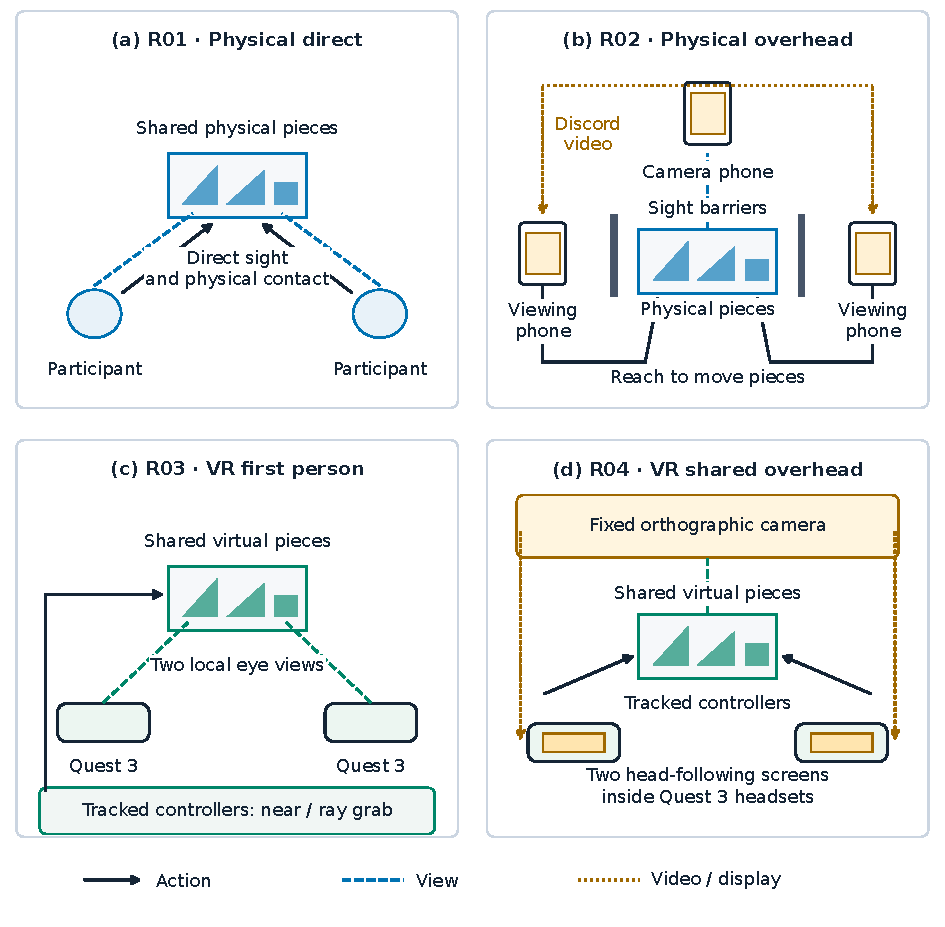
\includegraphics[width=\linewidth,height=140mm,keepaspectratio]{assets/figures/Figure3_2_apparatus.pdf}
\captionof{figure}[Apparatus and view mapping in the four study conditions (schematic, not to scale).]{Apparatus and view mapping in the four study conditions (schematic, not to scale). R02 uses one overhead camera phone and two participant viewing phones, with barriers blocking direct sight of the physical pieces. R03 provides local first-person views in two networked Quest 3 headsets. R04 displays the fixed overhead camera on a head-following screen inside each headset while retaining tracked controller manipulation. The VR schematic represents the shared-target collection arrangement used for G02--G06; the earlier G01 target arrangement is described in Section~\ref{sec:3-3}.}\label{fig:3-2}
\par\endgroup
\end{figureunit}

\begin{samepage}
In R01, physical direct viewing, participants looked directly at and moved seven physical pieces in the shared workspace. In R02, physical overhead video, one smartphone mounted above the table filmed the pieces. A Discord video call sent this live overhead feed to two other smartphones, one for each participant. Barriers blocked direct sight of the workspace. Participants watched their own phone while reaching into the shared physical workspace to move the real pieces. The setup changed visual access while retaining physical contact with the pieces. [\hyperlink{src:D24}{D24}, \hyperlink{src:D39}{D39}]
\par\end{samepage}

The two VR conditions used two networked Meta Quest 3 headsets running the Unity multiplayer Tangram prototype. Both participants manipulated the same seven virtual pieces using tracked controllers, with near and ray grabbing available. The host maintained the shared session and recorded the event stream. Software host and guest endpoints were mapped to the same participant numbers used in the recordings and questionnaires. [\hyperlink{src:D24}{D24}, \hyperlink{src:D39}{D39}, \hyperlink{src:D25}{D25}]

In R03, first-person VR, the participant viewed the scene from their own tracked perspective. In R04, shared overhead VR, a fixed orthographic camera provided a top view of the workspace on a virtual screen that followed the head and replaced the ordinary first-person scene. The screen was inside the headset. Controller tracking continued in the shared three-dimensional space, so the control mechanism remained spatial even though the displayed workspace was a top projection. [\hyperlink{src:D39}{D39}, \hyperlink{src:D40}{D40}, \hyperlink{src:D41}{D41}]

For the shared-target implementation used in the recorded G02--G06 sessions, both endpoints received the same world-oriented overhead image. Moving the head moved the display surface, but moving around the table did not rotate the overhead camera to match the participant. The target orientation, camera orientation and direction of the participant's own movements were therefore recorded as separate aspects of the setup. Participants sometimes changed position to find a more comfortable relation between what they saw and how they moved. This was a self-initiated adaptation described in the process records. [\hyperlink{src:D25}{D25}, \hyperlink{src:D41}{D41}, \hyperlink{src:D46}{D46}]

\par\addvspace{8pt}
\noindent\begin{minipage}{\linewidth}
\begingroup
\centering
\setstretch{1}
\fontsize{10}{12.3}\selectfont
\setlength{\tabcolsep}{2.2pt}
\renewcommand{\arraystretch}{1.18}
\captionof{table}[Implemented research conditions in fixed order.]{Implemented research conditions in fixed order.}\label{tab:3-1}
\begin{tabular}{@{}>{\raggedright\arraybackslash}p{13.729mm}>{\raggedright\arraybackslash}p{42.169mm}>{\raggedright\arraybackslash}p{101.009mm}@{}}
\toprule
\textbf{Round} & \textbf{Viewing} & \textbf{Manipulation and scope} \\
\midrule
R01 & Physical direct & Direct sight of a shared physical workspace; both partners move real pieces. \\
\addlinespace[3pt]
R02 & Physical overhead video & One overhead smartphone streams through Discord to two participant phones; barriers block direct sight; both move real pieces. \\
\addlinespace[3pt]
R03 & VR first person & Two Quest 3 headsets; local tracked views of shared virtual pieces; near and ray grabbing. \\
\addlinespace[3pt]
R04 & VR shared overhead & A world-fixed orthographic image appears on a head-following screen in each headset; controllers remain tracked in the shared 3D workspace. \\
\bottomrule
\end{tabular}
\par\endgroup
\end{minipage}\par\addvspace{8pt}




\section{Prototype changes and exposure history}\label{sec:3-3}

Target presentation changed during development. The first G01 recording used targets oriented to individual users. G02--G06 used the revised shared-target arrangement. The recorded configuration includes a fixed shared target, zero guest-specific optical rotation and manual ending without a time limit. After this iteration, G01 also experienced the full revised procedure. The pair preferred the new version but chose not to record the procedure again; their feedback is retained as a development observation. [\hyperlink{src:D43}{D43}, \hyperlink{src:D25}{D25}, \hyperlink{src:D74}{D74}]

Target patterns, VR experience and familiarisation varied between pairs. G01's candle-orientation discussion occurred during practice and informed development. G02's VR recordings were collected later using new target patterns that the pair had not previously solved. They are included with the other five pairs in the process analysis. Familiarisation was also part of the procedure for the other groups. [\hyperlink{src:D50}{D50}, \hyperlink{src:D17}{D17}, \hyperlink{src:D74}{D74}]

The original plan anticipated viewpoint switching. In the implemented formal rounds, the viewpoint remained locked to the designated condition. During G06's first-person candle task, a participant requested another view and the pair continued in first-person VR. View changes in preparation or between attempts form part of the exposure history. [\hyperlink{src:D14}{D14}, \hyperlink{src:D15}{D15}]



\chapter{Study and analysis method}\label{chap:4}

\section{Participants and study scope}\label{sec:4-1}

The study involved six dyads, identified as G01--G06, with twelve participants identified consistently as P01--P12. All pairs were already friends and had worked together; most were also members of a current course group, according to the researcher's final background clarification. Relationship duration and cooperation frequency were not measured. The study therefore describes collaboration between familiar partners. [\hyperlink{src:D18}{D18}]

Eight participants had previously used VR and four had not, according to the completed background record. One G05 participant had taken part in a Tangram club more than a decade earlier; the others were reported to have no Tangram experience. These reports describe prior exposure rather than current expertise. Participant numbers are retained across physical and VR conditions; viewing position is not used as a participant identity. [\hyperlink{src:D18}{D18}]

The study used an exploratory comparison with one designated process per pair and condition. All six pairs are included. Practice, restarts and additional experiences are recorded in the session history. G02's VR videos were recorded in a later session using previously unattempted target patterns, so the recorded tasks did not repeat a known solution. Their questionnaires describe the original session and are analysed as condition-level responses rather than ratings of individual recorded episodes. [\hyperlink{src:D17}{D17}, \hyperlink{src:D74}{D74}]


\section{Task and actual procedure}\label{sec:4-2}

Tangram provided a common task in which partners could refer to the same pieces, inspect a changing arrangement and decide together how to proceed. Retaining this task across the physical and VR arrangements kept the comparison focused on viewing and interaction within a common problem. Free manipulation allowed the pair to organise work at the level of a piece or local part, including changes between separate attempts and joint adjustment. This follows the interest in shared problem states and changing divisions of work described in collaborative learning and workspace-awareness research \cite{roschelle1995,dillenbourg1999,gutwin2002}. [\hyperlink{src:D72}{D72}, \hyperlink{src:D33}{D33}, \hyperlink{src:D36}{D36}, \hyperlink{src:D69}{D69}, \hyperlink{src:D38}{D38}]

Participants used seven Tangram pieces to construct target silhouettes. Both could manipulate the pieces, communicate naturally and decide how to divide work. The procedure did not assign a director or operator and did not require continuous think-aloud speech. Individual questionnaires followed the research rounds, and a recorded dyadic interview provided retrospective accounts. [\hyperlink{src:D38}{D38}]

All dyads experienced the conditions in the same order: R01, physical direct viewing; R02, physical overhead video; R03, first-person VR; and R04, shared overhead VR. Target patterns differed across rounds and were not balanced for difficulty. In G05, the chair was selected as a harder task after the pair performed well earlier. Comparisons therefore concern the task and viewing arrangements as implemented, including order, practice and pattern differences. [\hyperlink{src:D17}{D17}, \hyperlink{src:D44}{D44}]

The apparatus and viewing-to-action mapping are shown in Figure~\ref{fig:3-2}. R02 used three smartphones connected through Discord and barriers that blocked direct sight of the pieces. R03 and R04 used two networked Quest 3 headsets. In R04 the head-following display showed the world-fixed overhead image, while tracked controllers continued to operate in the shared virtual workspace. Section~\ref{sec:3-2} gives the full arrangement. [\hyperlink{src:D24}{D24}, \hyperlink{src:D47}{D47}, \hyperlink{src:D41}{D41}]

Familiarisation followed different entry criteria. Participants with VR experience could proceed when they felt ready. Novices were asked to complete a pattern and switch viewpoints during practice. Practice duration and control proficiency were therefore not standardised across participants. G04's two woman attempts preceded the formal overhead swimmer task as adaptation. G06's same-side positioning began during familiarisation before the formal first-person round. [\hyperlink{src:D18}{D18}, \hyperlink{src:D45}{D45}, \hyperlink{src:D14}{D14}]

The researcher reports that changes of participant position were self-initiated. Researcher intervention is recorded separately where it occurred. G04's physical direct round included structural feedback, encouragement to communicate and later confirmation of an earlier approach before the pair abandoned the task. G03's overhead chair included two structural hints before completion. Elsewhere, no-hint status follows the researcher's declaration; the absence of a hint in a log is not an independent audio verification of its absence. [\hyperlink{src:D46}{D46}, \hyperlink{src:D07}{D07}, \hyperlink{src:D59}{D59}]

Participants were instructed to use all seven pieces and match the target silhouette. After they announced completion, the researcher checked the configuration on site. A solution could be accepted with an internal partition different from the reference image. The analysis records this on-site judgment separately from subsequent geometric checking. Selected configurations were reconstructed during analysis to examine their outlines; the researcher identified a mismatch in the accepted G06 first-person candle while reviewing it as a focal observation, and reconstruction was used to check that observation. [\hyperlink{src:D18}{D18}, \hyperlink{src:D16}{D16}]


\section{Evidence corpus and provenance}\label{sec:4-3}

Data collection combined process records with participants' accounts because the study concerned both how collaboration developed and how it was experienced. Recordings and available system traces retained placements, responses and changes in control. Post-round ratings described particular aspects of the experience, and the final interview allowed participants to explain difficulties and decisions in their own terms. This combination followed the planning emphasis on behavioural activity, with completion measures used as context for understanding the task process. [\hyperlink{src:D36}{D36}, \hyperlink{src:D70}{D70}, \hyperlink{src:D73}{D73}]

The corpus is organised as six dyads across four research conditions, giving 24 group--condition cells. The completed source queue contains 26 researcher process reports, including multiple recordings or endpoints for some processes. This is a count of source reports, not independent trials. The reports cover all 24 cells, including the later G02 recordings on new target patterns. [\hyperlink{src:D17}{D17}]

The analysis combines researcher-prepared video observations and corrections, recordings of the task, six group interview texts, 48 confirmed post-round questionnaire responses and available Unity records. Video observations describe visible placements, body positions and how participants continued one another's work. VR event and pose records support the timing, piece identity and sequence of recorded manipulations. Interview text provides participants' retrospective accounts, while questionnaires describe their experience of each round. Selected frames and log sequences were checked against the source files; these targeted checks supplement the researcher's process reports. [\hyperlink{src:D17}{D17}, \hyperlink{src:D44}{D44}, \hyperlink{src:D20}{D20}]

All six physical overhead recordings (R02) have no usable audio, so these recordings support visible-action descriptions. VR recordings generally captured only the recording participant's own voice, and the other endpoint was used where available. A missing partner voice is treated as missing audio coverage. G04's formal overhead swimmer round is covered by \href{https://github.com/YiyangQin-UQ/REIT7841/blob/main/thesis/v1.1/materials/README.md\#d67}{V23} but not by the surviving \href{https://github.com/YiyangQin-UQ/REIT7841/blob/main/thesis/v1.1/materials/README.md\#d66}{V17} segment, and G06 has no recording from the other endpoint. Spoken content from researcher reports is presented as attributed paraphrase unless its wording and speaker have been checked. [\hyperlink{src:D19}{D19}]

The six interview texts combine speakers and contain transcription errors. The analysis uses group-level paraphrases where individual attribution cannot be established. Answers to questions about imagined viewing conditions are treated as participants' reflections on those scenarios. Supervisor correspondence and meeting transcripts inform the design history and rationale rather than the behavioural findings. [\hyperlink{src:D19}{D19}, \hyperlink{src:D44}{D44}]

\par\addvspace{8pt}
\noindent\begin{minipage}{\linewidth}
\begingroup
\centering
\setstretch{1}
\fontsize{10}{12.3}\selectfont
\setlength{\tabcolsep}{2.2pt}
\renewcommand{\arraystretch}{1.18}
\captionof{table}[Coverage of process reports and confirmed questionnaires.]{Coverage of process reports and confirmed questionnaires.}\label{tab:4-1}
\begin{tabular}{@{}>{\raggedright\arraybackslash}p{13.459mm}>{\raggedright\arraybackslash}p{45.183mm}>{\raggedright\arraybackslash}p{31.724mm}>{\raggedright\arraybackslash}p{34.608mm}>{\raggedright\arraybackslash}p{28.840mm}@{}}
\toprule
\textbf{Round} & \textbf{Condition} & \textbf{Dyads with process reports} & \textbf{Confirmed questionnaires} & \textbf{NA item entries} \\
\midrule
R01 & Physical direct & 6 & 12 & 1 \\
\addlinespace[3pt]
R02 & Physical overhead video & 6 & 12 & 1 \\
\addlinespace[3pt]
R03 & First-person VR & 6 & 12 & 0 \\
\addlinespace[3pt]
R04 & Shared overhead VR & 6 & 12 & 0 \\
\bottomrule
\end{tabular}
\par\endgroup
\end{minipage}\par\addvspace{8pt}

The 26 source reports cover 24 pair--condition cells. The two NA item values are Q01 for P08 in R01 and R02.


\section{Questionnaire and system records}\label{sec:4-4}

The questionnaire contains twelve study-specific items rated from 1 to 5, with an unable-to-judge or not-applicable option. The items cover identifying referred pieces, understanding intended locations, judging a partner's understanding, explaining locations, following partner activity, task progress, action timing, avoiding interference, movement, rotation, responsibility and solving together. They are interpreted separately. They are not a validated composite collaboration scale. Appendix B gives the full item wording and the item-level data. [\hyperlink{src:D20}{D20}]

The questionnaire dataset contains 48 confirmed responses: twelve participants each contributed answers for all four rounds. Forty-five responses came from the original export. For the remaining three, the researcher reported that the participants had confirmed their answers for the corresponding round were identical to the referenced response, and entered those confirmed values. The confirmation record preserves which response was used and when the clarification was recorded; the historical submission timestamps were retained. The two original not-applicable entries remain non-numeric. All 48 confirmed responses are included in the descriptive tables and figures. [\hyperlink{src:D20}{D20}]

Questionnaire comparisons were made item by item, first within each participant across rounds and then between partners. The twelve study-specific items were kept separate, with no composite collaboration score or significance testing. Ratings are used alongside the process records to describe the experience of a round; a round-level response is not assigned to a single episode within it. Appendix B provides the full item wording and confirmed values. [\hyperlink{src:D44}{D44}, \hyperlink{src:D20}{D20}]

The VR records were first segmented into software attempts using start, reset, pause, resume and end events. Each selected attempt was then linked to a research condition through its task, viewing condition and video--log anchors. Software round numbers were kept separate from R01--R04. For example, G06's retained overhead process is software R03 after an interrupted software R02, but remains research condition R04. Filenames containing TECHNICAL\_TEST were retained as recorded; the filename alone was not used to identify the dyad or decide whether a process was formal. [\hyperlink{src:D17}{D17}, \hyperlink{src:D15}{D15}, \hyperlink{src:D25}{D25}]

The collection-period V3 logging guide describes accepted grabs, movement onset, piece poses, release and post-release settling. Round-start metadata in the available revised-version logs specify approximately 10 Hz piece-pose sampling and 2 Hz participant-pose sampling, with a movement-onset threshold of 2 mm or 2 degrees. These are nominal logging settings; actual samples follow the recorded timestamps. Participant poses describe head and controller positions and orientations, rather than eye gaze. After release, the stream includes settling poses and a terminal event labelled stable\_0.3s or settle\_timeout\_2s. The timeout marks the end of the observation window and does not establish that the piece had become stationary. [\hyperlink{src:D25}{D25}]

For action timelines, each grab\_accepted event was paired with its piece\_release using the software round, piece ID and manipulation ID, and the endpoint identity and temporal order were checked. Requests, denied grabs and repeated selections were not counted as new successful holds. Forced release and interruption records were kept distinct from an ordinary release. The selected intervals were checked against the corresponding original CSV rows. They show when an endpoint held a piece; their duration and count do not measure understanding, effort or the value of a contribution. [\hyperlink{src:D25}{D25}, \hyperlink{src:D21}{D21}]

A configuration at an analysis time was reconstructed from the latest recorded pose for each piece at or before that time within the selected attempt. Eligible states came from initial placement, held-pose, release, settling-pose and settled records. This last-known-state rule retains post-release changes and avoids interpolating an unrecorded placement. The source event, row and age of each pose were kept with the reconstruction, and later events were checked before treating a selected state as persistent. A missing later update means no later change was recorded for that piece in the selected trace. [\hyperlink{src:D26}{D26}]

Video position, active task seconds and UTC or wall-clock time were retained as separate clocks. Pauses, resets and delayed manual ending were read from the software record. Distinctive visible manipulations and task boundaries provided local alignment anchors, with mappings stated for the selected case. For G06 and G03, repeated visible grabs were matched to the event records to establish the participant mapping. G03's P05 event reported at video 03:06 and the selected active-time log sequence retain their separate timestamps. This preserves the distinction between identifying the person and aligning a particular event. [\hyperlink{src:D21}{D21}, \hyperlink{src:D26}{D26}, \hyperlink{src:D06}{D06}]


\section{Analytic procedure and interpretation}\label{sec:4-5}

\begin{figureunit}{4-1}
Analysis began within each dyad and condition and followed connected episodes rather than isolated grabs. An episode began with a proposal, placement or problem relevant to the current arrangement, and followed the partner's response, subsequent manipulation and resulting configuration until the local issue changed, was resolved or was abandoned. The record separated the accessible view and target, who proposed and built a part, who later changed it, the before-and-after arrangement and the source of any correctness judgment. This attention to unfolding talk, action and artefacts was informed by interaction analysis \cite{jordan1995}. Figure~\ref{fig:4-1} summarises the analysis workflow. [\hyperlink{src:D44}{D44}, \hyperlink{src:D21}{D21}]

\par\begingroup
\centering
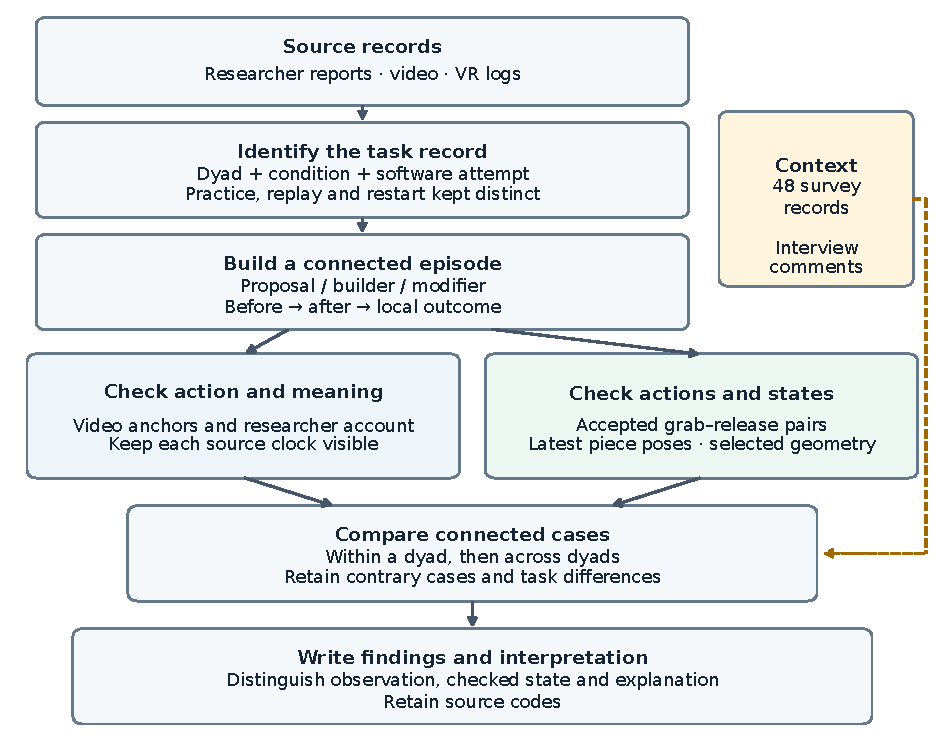
\includegraphics[width=\linewidth,height=125mm,keepaspectratio]{assets/figures/Figure4_1_analysis_flow.pdf}
\captionof{figure}[Analysis workflow.]{Analysis workflow. Source identification precedes episode construction so that software attempts, research conditions and recording sessions are identified consistently. Video and researcher accounts describe the meaning and order of local actions; accepted event pairs and reconstructed states check selected movements and configurations. Questionnaire responses and interview comments provide context for the case comparison. The separation between source-specific clocks, on-site acceptance and later geometric verification is retained in the findings.}\label{fig:4-1}
\par\endgroup
\end{figureunit}

Researcher observations and subsequent corrections provided the initial event accounts. Selected video frames and log intervals were then checked to examine the reported order of actions, the pieces involved and the resulting arrangement. Grounding and workspace awareness served as sensitising concepts when interpreting reference, response, coordination and assistance \cite{clark1991,gutwin2002}. The operational distinctions in Appendix C describe local uptake, parallel and complementary work, preservation, self-revision, partner revision and manipulation difficulty. Table~\ref{tab:C-2} shows three worked applications with their original time bases. [\hyperlink{src:D44}{D44}, \hyperlink{src:D21}{D21}]

Processes were compared first across conditions within a dyad and then across dyads. Cases were selected for detailed presentation when the relevant sequence could be traced and when they clarified a question raised by the other records. These included configurations that looked plausible during the task, shifts in who developed a part, preservation of a partner's arrangement, self-revision and active partner intervention. G06's candle connects configuration change with shared rebuilding; G01 and G03 provide distinct self-revision sequences. Action and response support an interpretation of a local step, while an intention or reason for preserving it requires the surrounding account. [\hyperlink{src:D17}{D17}, \hyperlink{src:D21}{D21}]

The comparison across pairs used a process criterion: participants formed an arrangement that resembled the target as a whole while a piece remained unused, or while the contour or proportions still differed from the target after all seven pieces had been used. Ordinary unfinished search and difficulty placing an individual piece were recorded separately. Each pair contributed one presence judgment per condition. The researcher identified this pattern in three of six first-person VR records and in none of the six shared-overhead VR records. Table~\ref{tab:A-3} links each pair to the relevant records. [\hyperlink{src:D27}{D27}, \hyperlink{src:D74}{D74}]

The geometric checks were conducted after data collection. For selected VR states, the saved Unity piece meshes and scale were combined with the logged world positions and quaternion rotations. Vertices were projected onto the tabletop x--z plane and reduced to a convex hull for each piece, preserving the recorded arrangement and the mesh's rounded geometry. The saved scene supplied the mesh geometry, while the CSV supplied the pose at each time. Comparison panels retained a common world scale and used rigid alignment of whole arrangements. They were checked alongside the target image, video frames and process reports. [\hyperlink{src:D26}{D26}, \hyperlink{src:D16}{D16}]

For the candle comparison, the researcher first noticed that the accepted construction's outline differed from the target. Reconstructed top views placed the target and recorded configurations in a common orientation so that this difference could be inspected. A simple comparison of corresponding upper and lower spans was used as a supporting check: they are equal in the target and in the two-large-triangle layouts, whereas G06's lower span is wider. The reconstruction preserves each piece's recorded position and rotation. Numerical measurements and processing details are retained with the figure sources. [\hyperlink{src:D26}{D26}, \hyperlink{src:D16}{D16}, \hyperlink{src:D74}{D74}]

The researcher identified the focal observations, selected the cases and developed the interpretations from the study records. AI-assisted processing helped check selected sequences and geometric relations, organise the source material and prepare figures and prose. The G06 outline mismatch was an observation made by the researcher and subsequently checked through reconstruction. [\hyperlink{src:D44}{D44}, \hyperlink{src:D21}{D21}, \hyperlink{src:D74}{D74}]




\section{Consent and research assistance}\label{sec:4-6}

The study was undertaken as an educational activity for the thesis course. Twelve completed participant consent forms are retained in the local archive. In correspondence dated 6 October 2026, the supervisor confirmed that the previous testing could be used because the study had been reviewed for an educational activity rather than a research publication output. Participant codes are used in this report, and the task-image excerpts focus on the workspace and hands. [\hyperlink{src:D22}{D22}]

ChatGPT and Codex supported source organisation, English drafting and revision, log and geometric checks, programmatic figures and typesetting. The researcher conducted the study, identified the findings and judged the interpretations. The AI-use statement records this assistance by project stage. [\hyperlink{src:D23}{D23}, \hyperlink{src:D74}{D74}]



\chapter{Results}\label{chap:5}

The six pairs organised their Tangram work through local attempts, suggestions, placements and revisions. Three connected findings emerged from the process records. First, a construction that resembled the target could conceal an unused piece or an incorrect proportion. Second, the division of work changed as participants encountered dependencies between parts of the construction. Third, an existing partial solution could be preserved by a partner and later revised by the person who had built it. Together, these findings connect the geometry visible in the workspace with the actions through which pairs developed and accepted a solution.

The analysis draws primarily on the researcher's video process records and the VR action and pose logs. Video records establish the sequence of proposals, responses and visible actions. Logs identify the manipulated pieces and record their positions, rotations, grabs and releases. The figures use these sources to show both the development of an arrangement and the people who changed it. Participants are identified by their P01--P12 codes throughout. Video timestamps locate events in a recording; active log seconds locate events within a research round.

\section{Plausible shapes and overlooked geometric problems}\label{sec:5-1}

In first-person VR, three of the six pairs produced a near-complete arrangement with an unused piece, or an arrangement using all seven pieces whose outline or proportions did not match the target. These were G01, G05 and G06. In the researcher's process records, none of the six pairs showed the same pattern in shared-overhead VR. The pattern concerns an arrangement that already resembled the target. Difficulty finding a solution, or having pieces left while a construction was still incomplete, was treated separately. Table~\ref{tab:5-1} shows how the three first-person cases developed and how their outcomes differed.

\par\addvspace{8pt}
\noindent\begin{minipage}{\linewidth}
\begingroup
\centering
\setstretch{1}
\fontsize{10}{12.3}\selectfont
\setlength{\tabcolsep}{2.2pt}
\renewcommand{\arraystretch}{1.18}
\captionof{table}[Near-complete shape problems in first-person VR.]{Near-complete shape problems in first-person VR. These are three cases within the six pairs, as identified in the researcher's process records.}\label{tab:5-1}
\begin{tabular}{@{}>{\raggedright\arraybackslash}p{16.614mm}>{\raggedright\arraybackslash}p{62.763mm}>{\raggedright\arraybackslash}p{77.531mm}@{}}
\toprule
\textbf{Pair} & \textbf{Problem in candidate} & \textbf{Response and outcome} \\
\midrule
G01 & Chair outline formed with the medium triangle unused. & Replacement was attempted and rejected when edges did not align. \\
\addlinespace[3pt]
G05 & All seven pieces formed a chair with an elongated proportion. & A partner questioned the result; revision continued. \\
\addlinespace[3pt]
G06 & Six-piece candle with the medium triangle unused, followed by rebuilding. & Seven-piece result accepted during the session; later reconstruction showed a proportion mismatch. \\
\bottomrule
\end{tabular}
\par\endgroup
\end{minipage}\par\addvspace{8pt}

G01 built a plausible chair outline while the medium triangle remained outside it. P02 brought the remaining piece to the partner's attention. The pair also adjusted access to the target: P01 lifted a large triangle to see the reference, and the arrangement was moved to make space around the silhouette. They then tried substituting the medium triangle for a smaller piece. The edges did not align, and the attempt was rejected. The handling of the pieces therefore served different purposes within one sequence: exposing the reference, displaying a problem and testing a candidate solution. [\hyperlink{src:D04}{D04}]

G05 reached a seven-piece chair whose proportions were too long. A partner questioned its match with the target, and exploration continued. The subsequent construction involved changing the role of the parallelogram between the seat and backrest. G05 thus provides a case in which a plausible whole was questioned during the task. G01 rejected a candidate when the replacement failed, whereas G06 accepted a final configuration whose geometric problem was identified later. [\hyperlink{src:D10}{D10}]

\subsection{G06 from a six piece candidate to accepted completion}\label{sec:5-1-1}

G06's candle provides the clearest link between the construction process and the later geometry check. P11 initially worked mainly on the body, while P12 worked on the top. Six pieces formed a recognisable candle, leaving the medium triangle unused. The pair tried to incorporate it, opened the body and developed another internal arrangement. The medium triangle was eventually included, and both participants accepted the seven-piece result. The researcher also accepted it during the session. [\hyperlink{src:D14}{D14}]

\begin{figureunit}{5-1}
Figure~\ref{fig:5-1} reconstructs six stages from the recorded piece poses. At 45 active log seconds, six pieces formed the candidate and the medium triangle remained outside it. The 64-second state shows an attempt to use the medium triangle; the 83-second state shows the body opened. By 145 seconds, the arrangement included a new large-triangle anchor. The medium triangle had been incorporated by 184 seconds, and the 214-second state shows the seven-piece configuration accepted at the end of the process. These states make the changes to the construction visible alongside the researcher's account.

\par\begingroup
\centering
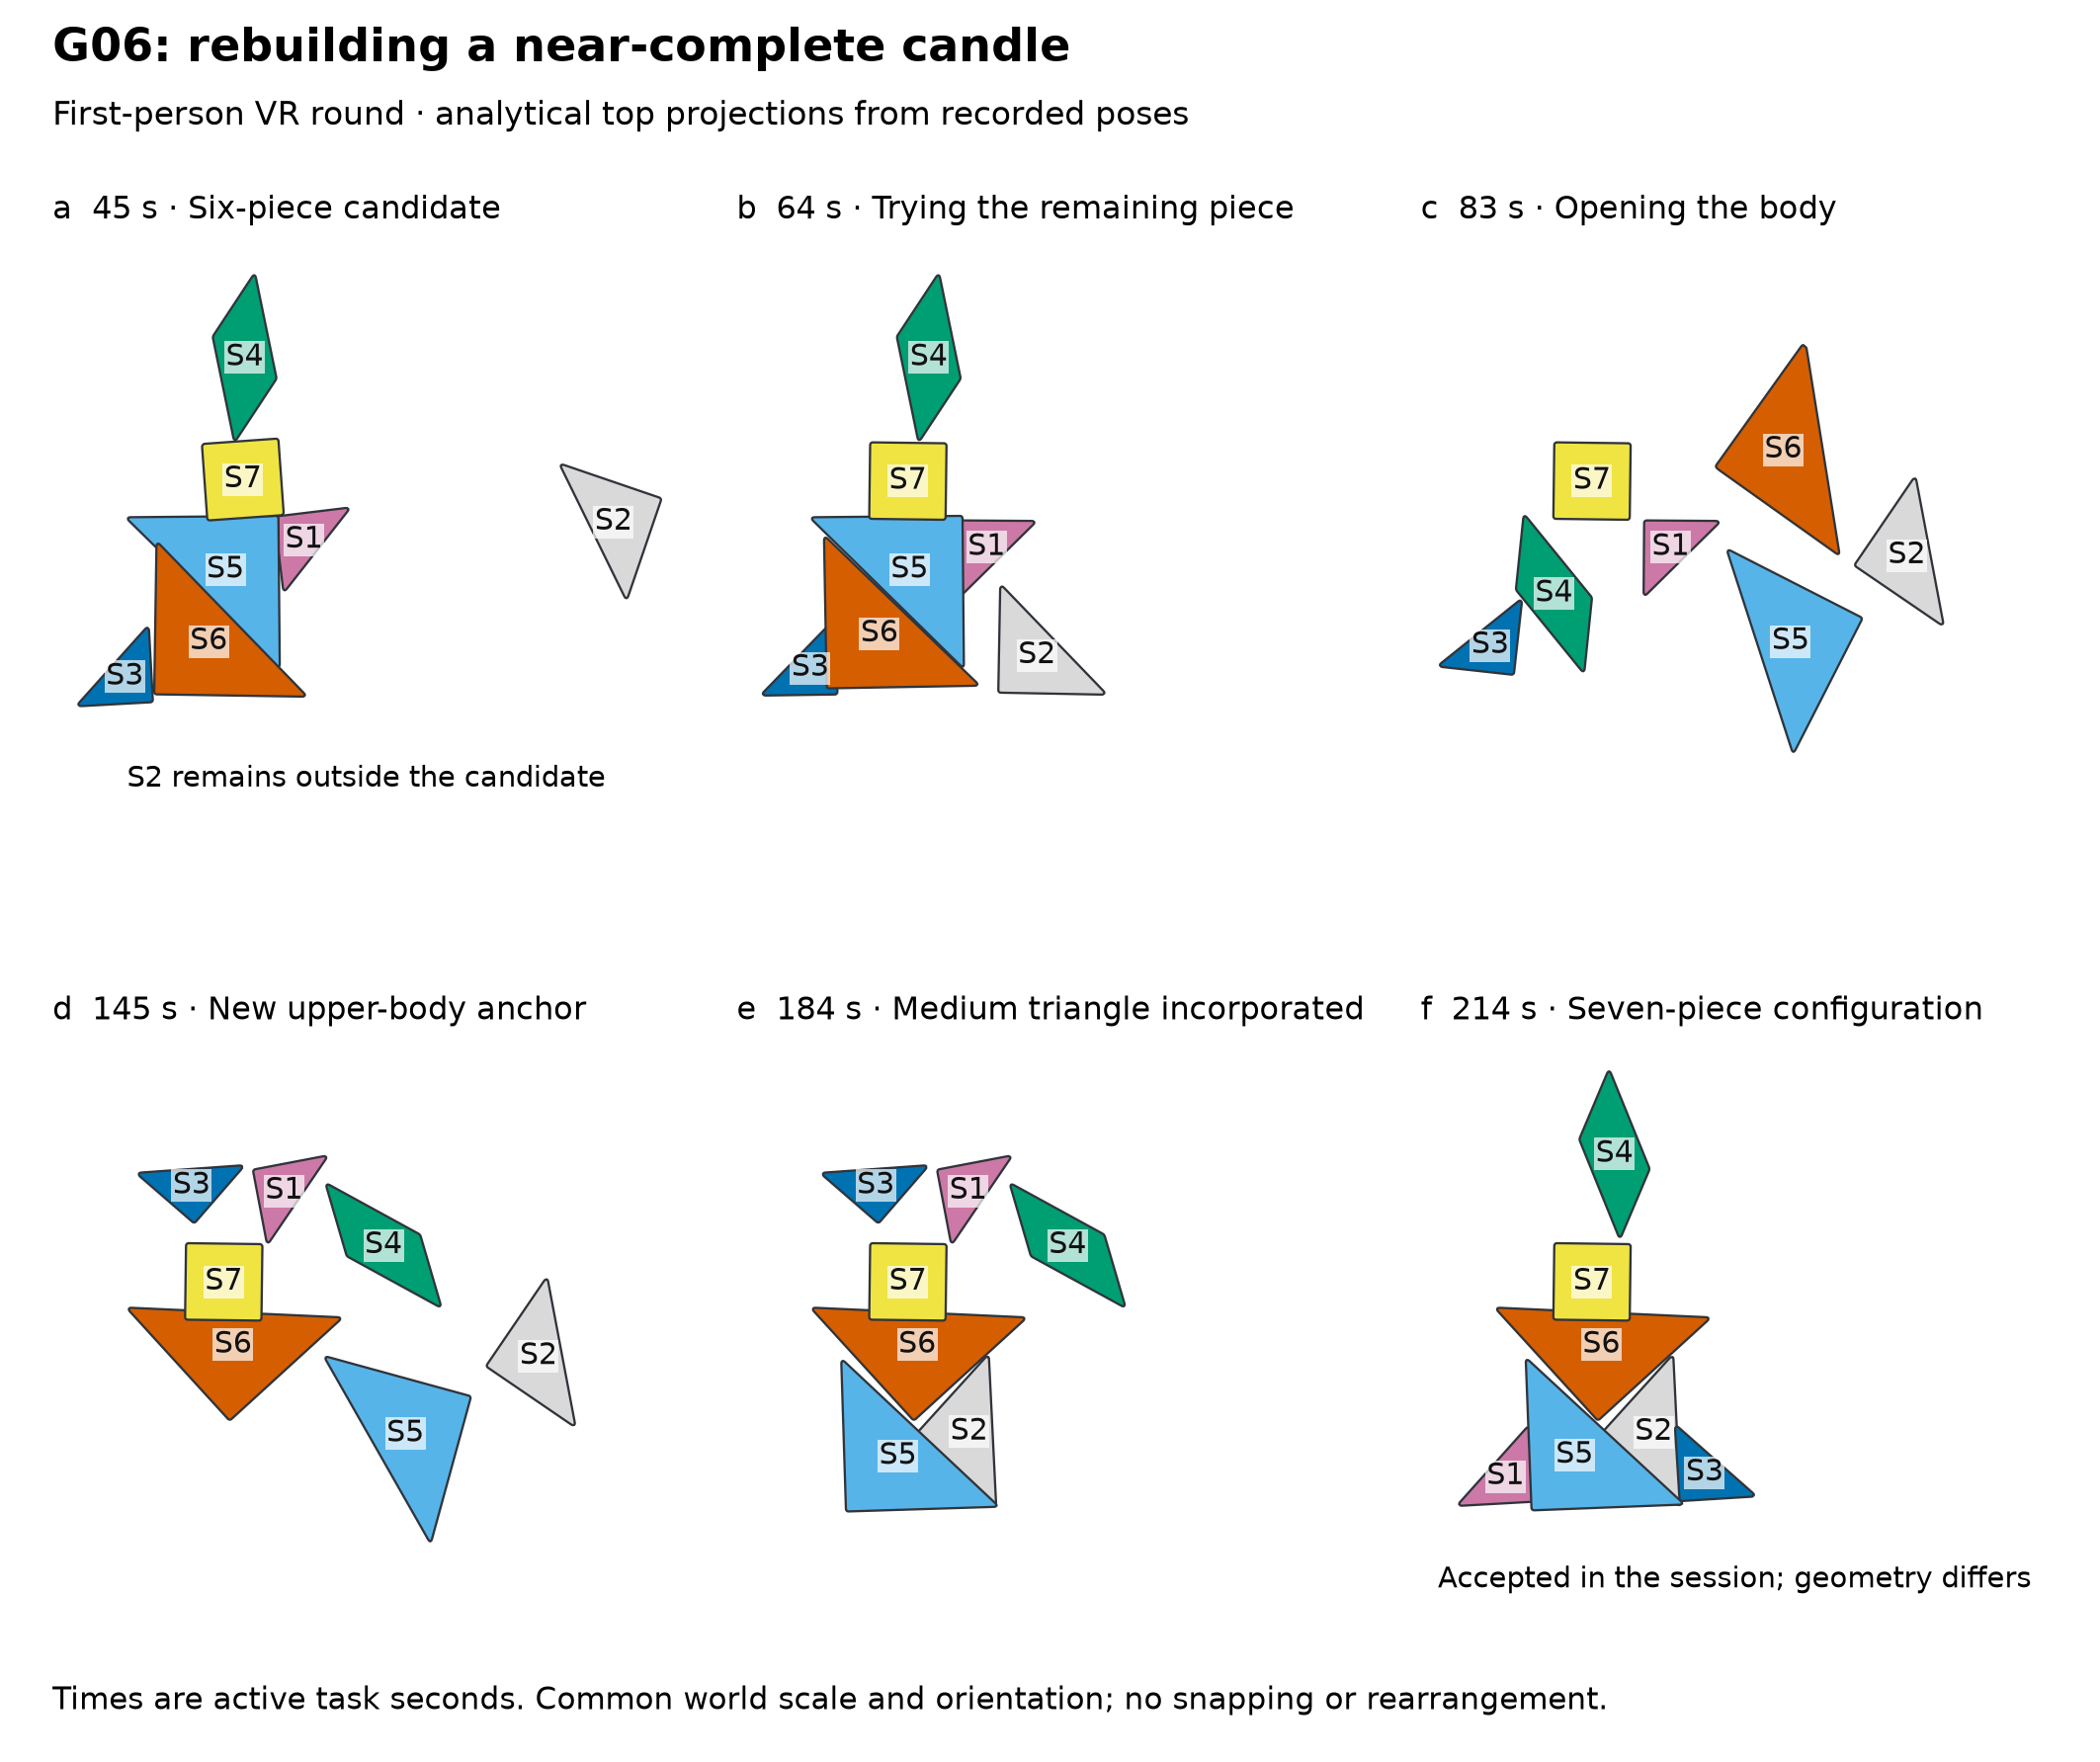
\includegraphics[width=\linewidth,height=134mm,keepaspectratio]{assets/figures/fig01_g06_reconstruction_sequence.png}
\captionof{figure}[G06's candle at six active-task times, reconstructed from the saved piece mesh and recorded poses.]{G06's candle at six active-task times, reconstructed from the saved piece mesh and recorded poses. Every panel has the same scale and world orientation. S2 is the medium triangle. No piece was snapped or rearranged. The video process record establishes acceptance of the final configuration; the logs establish the geometry. These analytical top projections were not participant views. The final outline is examined in Figures~\ref{fig:5-2} and~\ref{fig:5-3}. [\hyperlink{src:D14}{D14}]}\label{fig:5-1}
\par\endgroup
\end{figureunit}



While rebuilding the candle during the task, P11 asked to try another viewpoint, at approximately 13:46 in the available recording. View switching was locked during the formal round, so the pair continued in first-person VR. The request places viewing conditions within the participants' own efforts to resolve the task. The view remained first-person throughout the formal round. [\hyperlink{src:D14}{D14}]


\subsection{Reconstructing the accepted geometry}\label{sec:5-1-2}

\begin{figureunit}{5-2}
The researcher noticed that the accepted G06 candle was wider at the bottom than the target. Figure~\ref{fig:5-2} places the recorded first-person view beside the reconstruction, making the outline mismatch visible. Figure~\ref{fig:5-3} compares it with the target and two other first-person candle constructions. G03 and G04 use two equal large triangles for the corresponding upper and lower spans; G06 uses a different combination with a wider lower body. A supporting span comparison gives approximately 1.39 for G06 against 1.00 for the target and the other two constructions. These top views were reconstructed after the tasks to check the researcher's observation. [\hyperlink{src:D16}{D16}, \hyperlink{src:D74}{D74}]

\par\begingroup
\centering
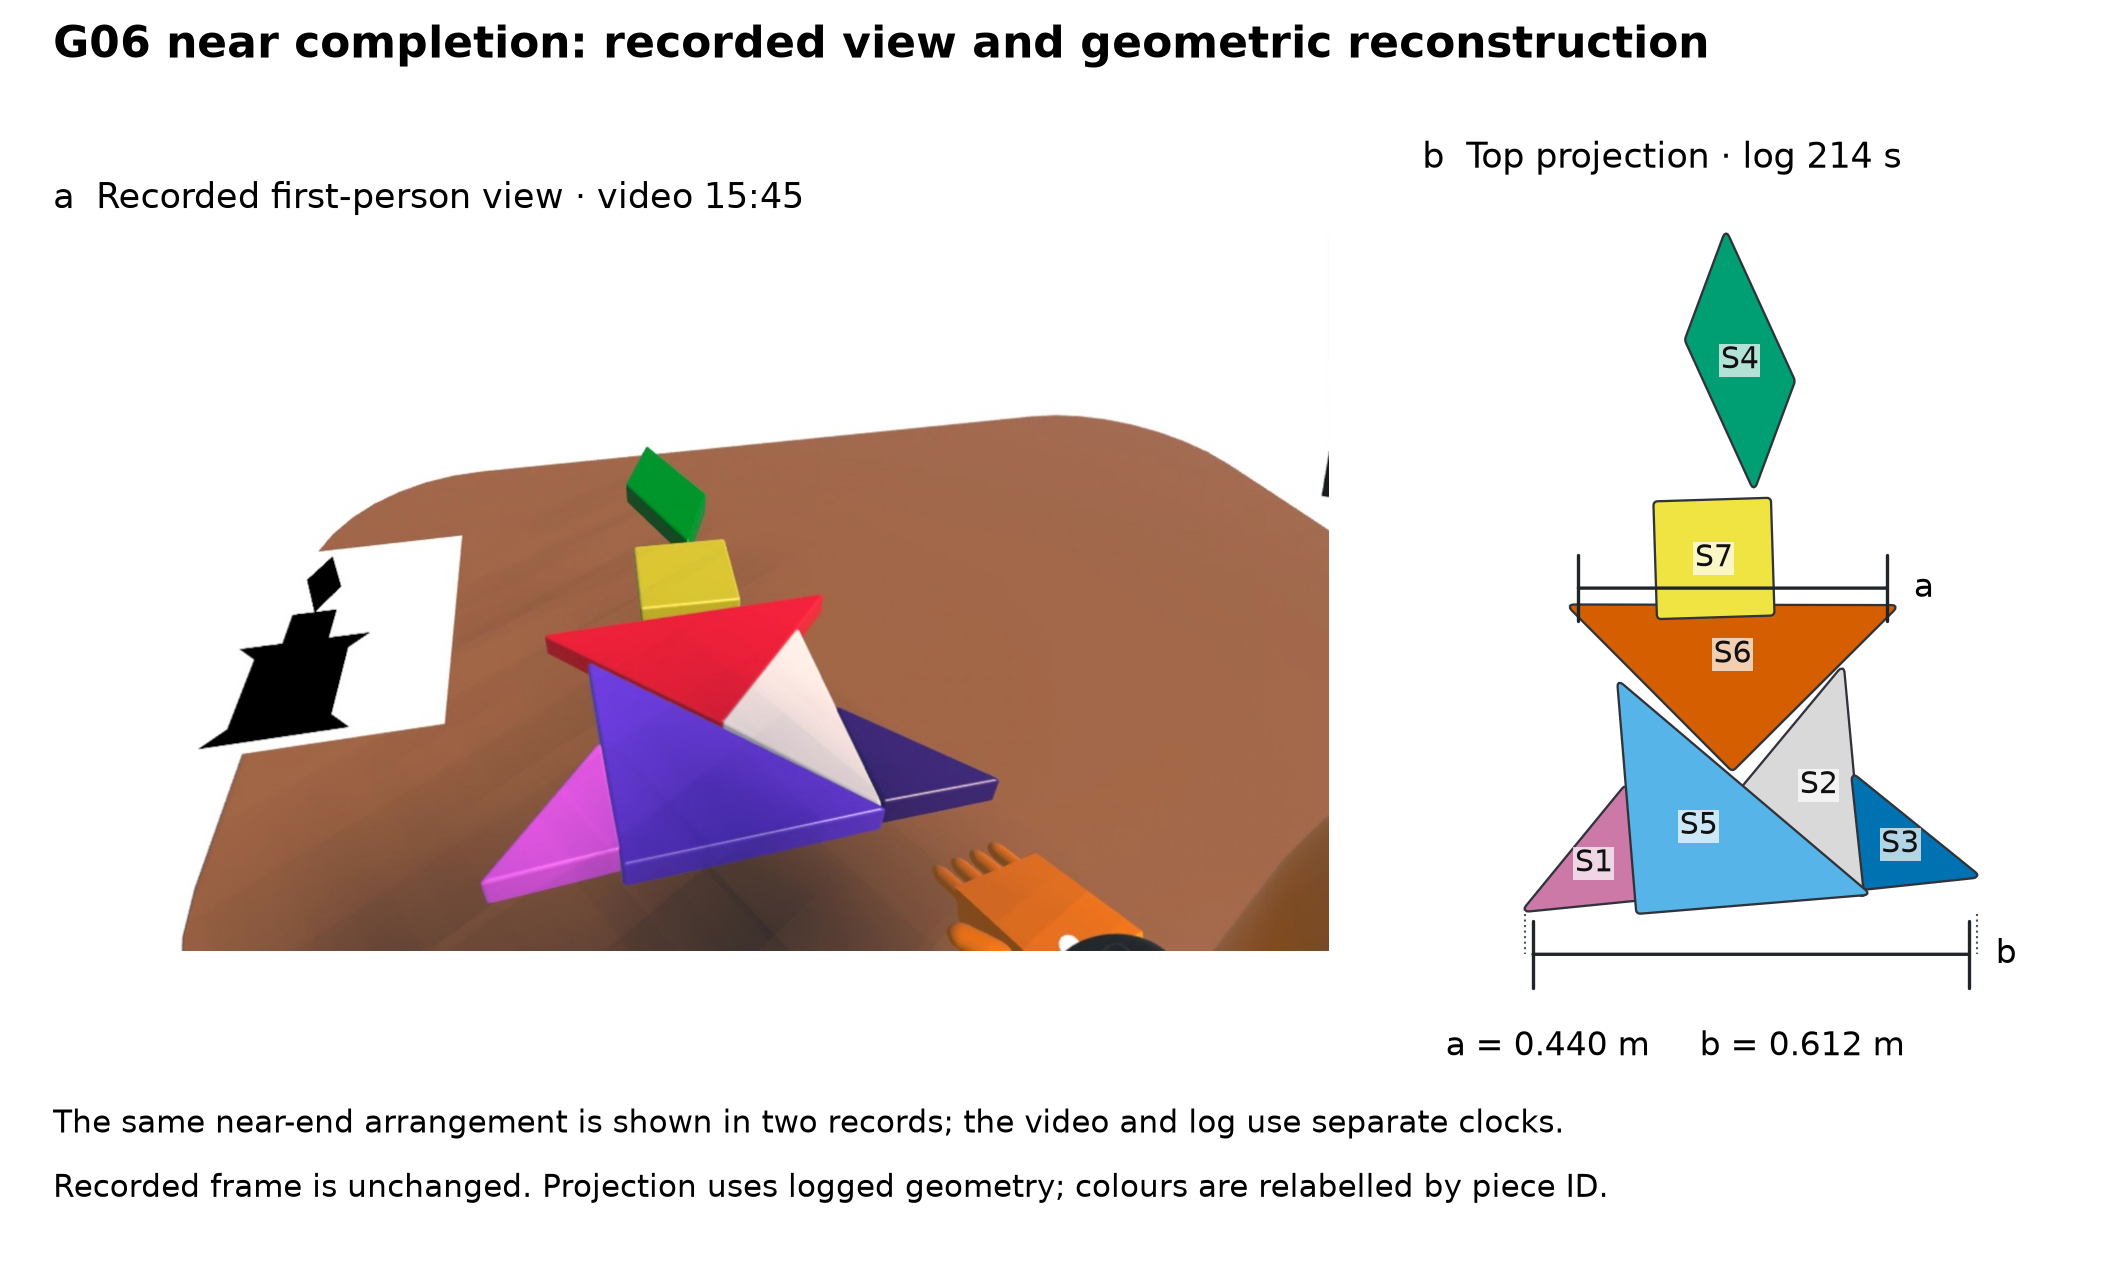
\includegraphics[width=\linewidth,height=153mm,keepaspectratio]{assets/figures/fig03_g06_recorded_view_and_geometry.png}
\captionof{figure}[The near-end G06 arrangement in a recorded first-person frame at 15:45 (left) and a reconstruction at 214 active-task...]{The near-end G06 arrangement in a recorded first-person frame at 15:45 (left) and a reconstruction at 214 active-task seconds (right). These are independent video and log clocks, showing the same near-end arrangement rather than frame-exact synchronisation. The reconstruction uses colours assigned by piece ID. Dimension a is the upper large triangle's longest projected chord; b is the lower-piece span along that direction. This is an analytical comparison, not an in-task switch to overhead viewing. [\hyperlink{src:D14}{D14}, \hyperlink{src:D16}{D16}]}\label{fig:5-2}
\par\endgroup
\end{figureunit}



\begin{samepage}
The recorded first-person view and the log-based reconstruction show the near-end arrangement on their respective time bases. The reconstruction makes the unequal spans directly inspectable. In an oblique view, the apparent lengths and angles depend on viewing direction and distance; a perpendicular orthographic view preserves the shape of the planar arrangement. The case therefore connects an observed judgment during collaboration with a specific geometric mismatch. Section~\ref{sec:6-1} considers what this relationship means for viewpoint design.
\par\end{samepage}

\begin{figureunit}{5-3}
\par\begingroup
\centering
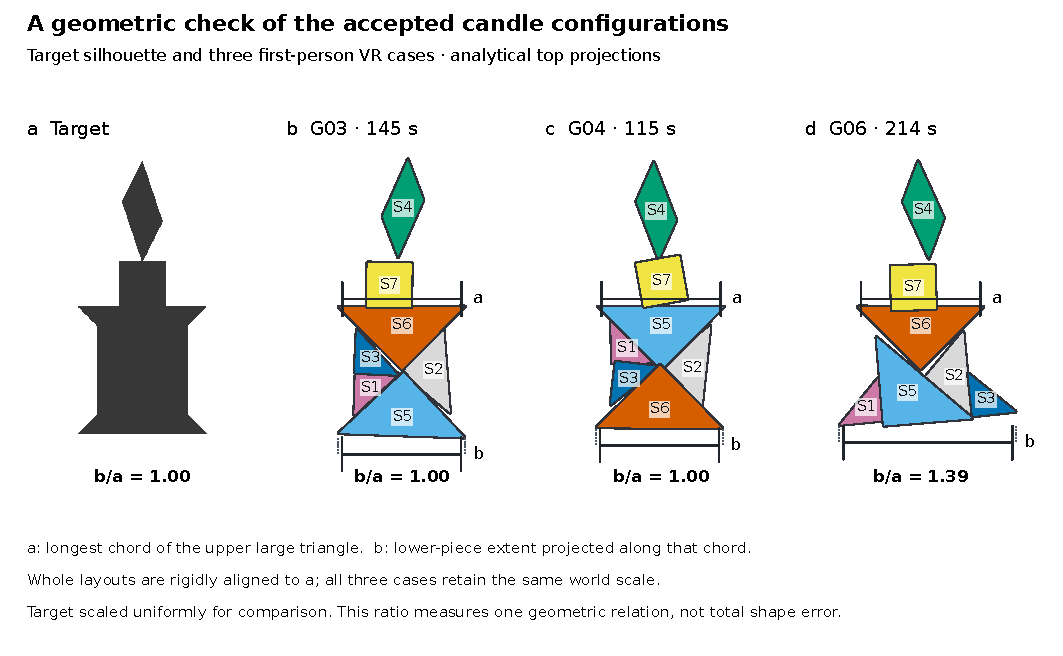
\includegraphics[width=\linewidth,height=153mm,keepaspectratio]{assets/figures/fig02_candle_geometry_comparison.pdf}
\captionof{figure}[Target silhouette and three first-person VR configurations.]{Target silhouette and three first-person VR configurations. Entire layouts are translated and rigidly rotated to align a; individual piece relations and world scale are preserved. The lower span b uses one large triangle in G03 and G04, and S1/S5/S3 in G06. The displayed span ratios are 1.00, 1.00 and 1.39, respectively. The target silhouette is scaled uniformly for display. This ratio measures one width relation, not total shape error. Rounded mesh corners and thickness are retained. [\hyperlink{src:D16}{D16}, \hyperlink{src:D06}{D06}, \hyperlink{src:D08}{D08}, \hyperlink{src:D14}{D14}]}\label{fig:5-3}
\par\endgroup
\end{figureunit}




The two pieces of evidence address complementary questions. The condition-level process records identify where the near-complete shape problems occurred. The G06 reconstruction identifies a measurable mismatch in a particular accepted construction. The fixed sequence, different target patterns and prototype versions remain part of the condition comparison; the examples establish the practical relevance of geometric presentation within the studied tasks.


\section{Expressing ideas and continuing shared constructions}\label{sec:5-2}

Participants expressed local ideas through placements that their partners could inspect, continue or change. Who advanced a part could change during the round, and both participants could return to an arrangement when the remaining pieces did not fit. The process records and action logs trace how these contributions connected within the shared task.

\begin{samepage}
In G06's first-person candle, the initial body-and-top arrangement became a shared reconstruction problem when the medium triangle remained unused. Both participants subsequently manipulated the body. The logged sequence in Figure~\ref{fig:5-4} shows who handled each piece and when. It makes the move from separate local work to repeated intervention in the same set of pieces inspectable. The six reconstructed states in Figure~\ref{fig:5-1} show what those actions produced. Read together, the two figures connect a change in work organisation to the changing configuration, rather than treating all grabs as equivalent contributions.
\par\end{samepage}

\begin{figureunit}{5-4}
\par\begingroup
\centering
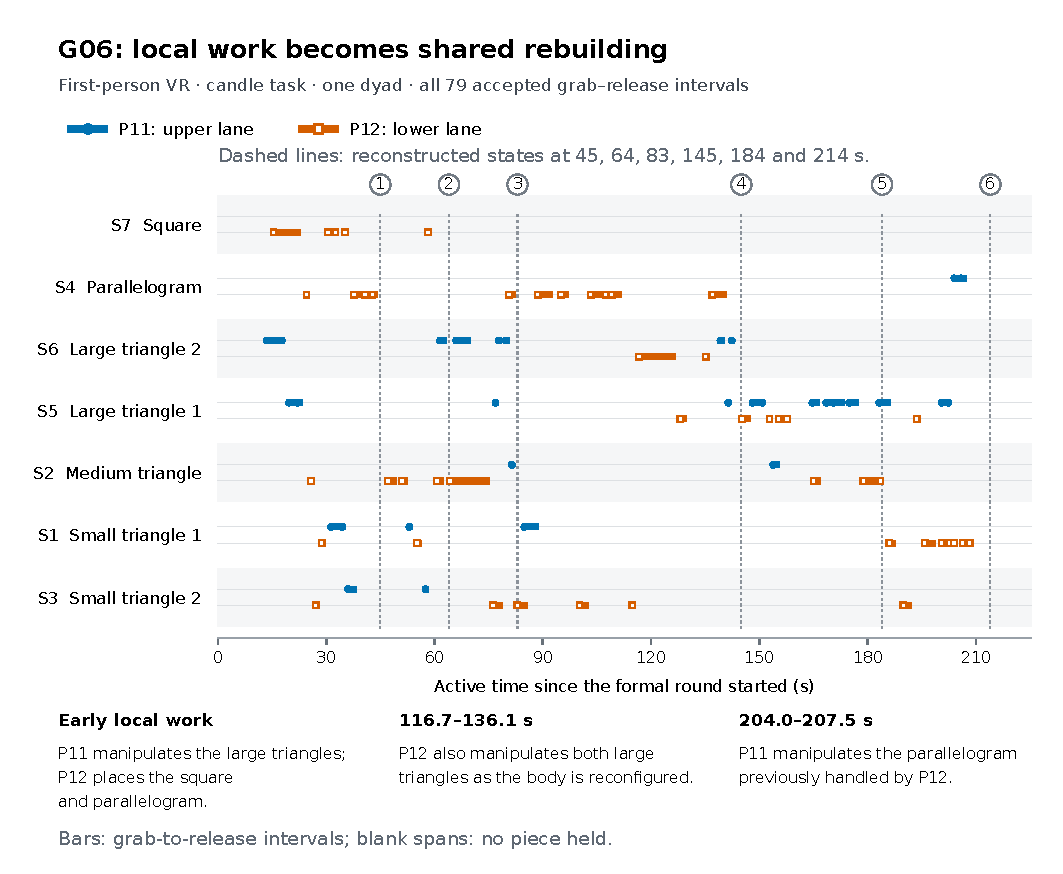
\includegraphics[width=\linewidth,height=132mm,keepaspectratio]{assets/figures/F3_G06_action_timeline.pdf}
\captionof{figure}[All 79 logged manipulation intervals in G06's first-person candle round.]{All 79 logged manipulation intervals in G06's first-person candle round. P11 is the upper lane and P12 the lower lane for each piece. A segment runs from accepted grab to release; its marker identifies the grab. Vertical guides match the six states in Figure~\ref{fig:5-1}. Later actions cross the initial body/top division: P12 handles both large triangles and P11 handles the parallelogram. Object control does not measure idea ownership or relative contribution. Participant identities follow the recording-position mapping and checked endpoint alignment. [\hyperlink{src:D14}{D14}]}\label{fig:5-4}
\par\endgroup
\end{figureunit}

\begin{samepage}
The change is visible at piece level. P11 first grabbed large triangle S6 at 13.58 active seconds, while P12 handled square S7 from 15.40 to 22.87 seconds. Later, P12 manipulated S6 from 116.67 to 126.75 seconds and the other large triangle, S5, from 128.07 to 129.79 seconds. Between 145.14 and 158.71 seconds, S5 was manipulated in sequence by P12, P11 and P12. Near the end, P11 manipulated the parallelogram S4 in two intervals, 204.03--204.90 and 205.89--207.47 seconds, after P12 had handled it earlier. These changes show the initially separate work on the body and top becoming repeated manipulation of the same pieces by both partners. [\hyperlink{src:D14}{D14}]
\par\end{samepage}



G03's candle developed through a different sequence. P05 proposed using two small triangles for the flame, while P06 used the parallelogram for that part. P06 invited P05 to move to the same side of the table, and P05 did so. The pair still pursued different flame constructions. At approximately 03:06 in P05's recording, P05 dismantled the two-small-triangle arrangement and used those pieces for the base. P06 later continued the solution, and the candle was completed. The source records show overlapping local attempts followed by a reallocation of both pieces and work. Their common viewing position preceded the resolution of the different construction ideas. [\hyperlink{src:D06}{D06}]



\begin{samepage}
The G03 logs also provide a direct trace of self-revision followed by partner continuation (Figure~\ref{fig:5-5}). By 52 active seconds, P05 had brought small triangles S1 and S3 together. P05 grabbed them again at 67.38 and 69.33 seconds; the 73-second reconstruction shows them separated. P06 subsequently grabbed S3 at 93.56 seconds and S1 at 96.29 seconds. The 99-second state shows the resulting changes. The same pieces therefore passed from one person's local arrangement, through that person's revision, to manipulation by the partner. The endpoint-to-participant mapping was checked against three visible grabs in the recording. The video account supplies the interpretations of flame and base; its reported event and the selected log snapshots are shown at their respective recorded times. [\hyperlink{src:D06}{D06}]
\par\end{samepage}

\begin{figureunit}{5-5}
\par\begingroup
\centering
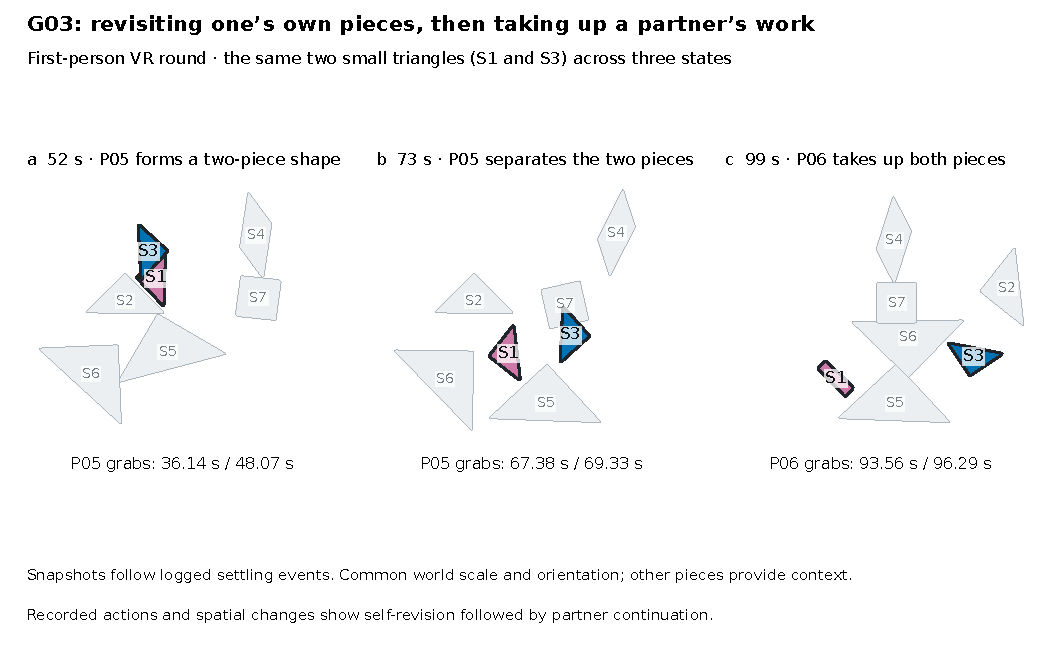
\includegraphics[width=\linewidth,height=100mm,keepaspectratio]{assets/figures/fig04_g03_self_revision_and_continuation.pdf}
\captionof{figure}[G03 configurations at 52, 73 and 99 active seconds, with the same scale and orientation.]{G03 configurations at 52, 73 and 99 active seconds, with the same scale and orientation. S1 and S3 are highlighted; other pieces show context. P05 brings them together, later separates them, and P06 subsequently operates on both. The snapshots follow settling events at 51.522, 72.518 and 98.699 seconds. S1 is nearly edge-on in the last projection because its recorded three-dimensional pose is retained. These selected states show self-revision followed by partner continuation; intermediate actions remain in the source event list. [\hyperlink{src:D06}{D06}]}\label{fig:5-5}
\par\endgroup
\end{figureunit}

In G01's physical direct-view chicken task, P02 questioned P01's proposed use of a large triangle for the back at approximately 00:34. P01 continued the attempt. Around 01:05, P02 began trying the alternative by fitting the medium and large triangles together. The researcher reported that P01 then accepted this arrangement and moved to other parts around 01:20. At 01:25, P01 proposed using a small triangle for the head; P02 added the square beneath it at 01:27, and P01 straightened it. The sequence moved from disagreement about a local part to an enacted alternative, followed by work on the next part. [\hyperlink{src:D01}{D01}]

\begin{figureunit}{5-6}
In G06's physical overhead goose task, P12 initially placed the square as the head. P11 added a small triangle and the parallelogram for the mouth and neck. At approximately 00:33, P11 tried to establish the body's large-triangle arrangement without resolving it. P12 continued from the existing neck by adding a small triangle at 00:53. P11 placed the medium triangle against it at 01:02. From approximately 01:11, both participants placed the remaining large triangles, and the researcher recorded successful completion at 01:20. During the subsequent reference check, their solution had a different internal partition: the head region combined the square and a small triangle, while the reference used the medium triangle and a small triangle, with the other combination in the corresponding body region. Figure~\ref{fig:5-6} shows the successive additions and the later reference check. [\hyperlink{src:D12}{D12}]

\par\begingroup
\centering
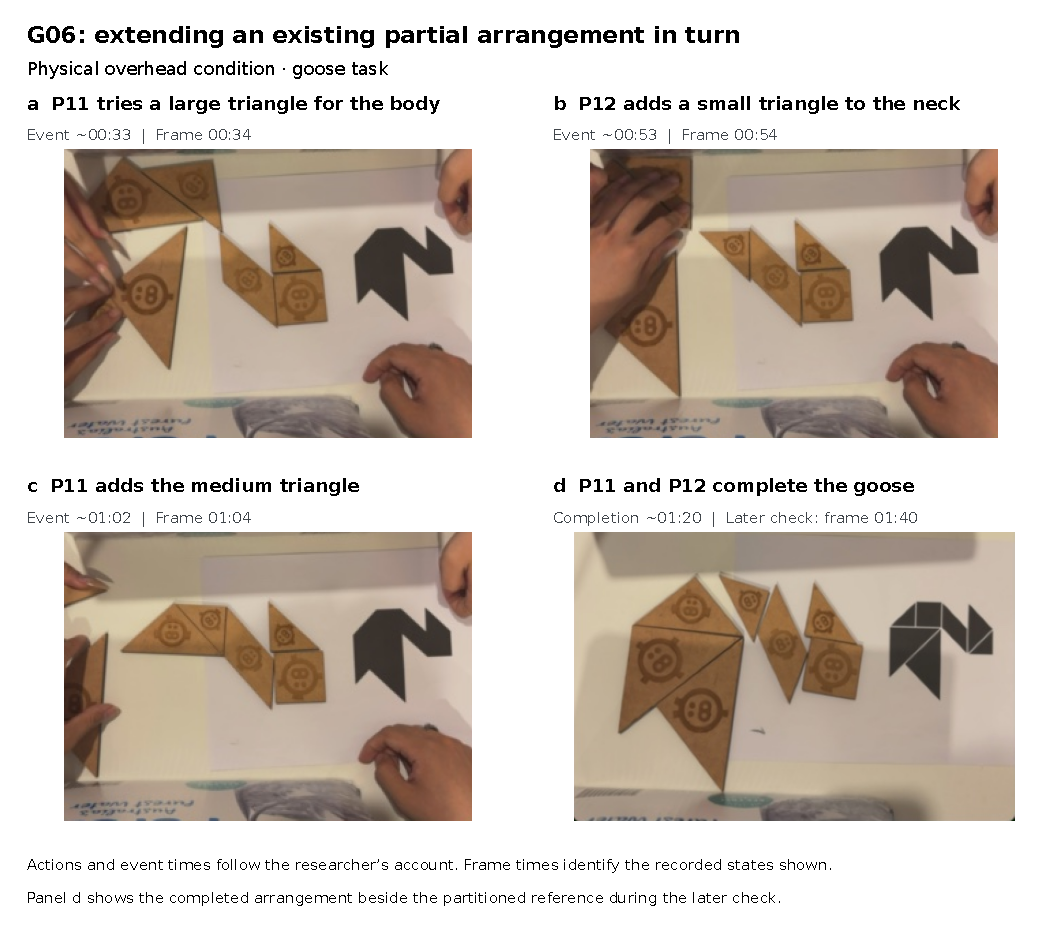
\includegraphics[width=\linewidth,height=115mm,keepaspectratio]{assets/figures/fig07_g06_goose_continuation.pdf}
\captionof{figure}[G06 extending a partial goose arrangement in the physical overhead condition.]{G06 extending a partial goose arrangement in the physical overhead condition. The researcher's process account records P11 trying a large triangle for the body (a, approximately 00:33), P12 adding a small triangle to the existing neck (b, 00:53), and P11 continuing with the medium triangle (c, 01:02). Both participants then placed the remaining large triangles and completed the goose at approximately 01:20. Panel d shows the later reference check at 01:40. The completed arrangement uses a different internal partition from the reference: the square and medium triangle occur in different regions, each paired with a small triangle. Event times and actor attribution follow the researcher's account; frame times identify the displayed video images. [\hyperlink{src:D12}{D12}]}\label{fig:5-6}
\par\endgroup
\end{figureunit}



\begin{samepage}
In the G06 interview, one participant described treating the partner's not removing their placed pieces as a sign that the partner understood what they were doing. In response to a discussion of the task's division into parts, the transcript also records a participant describing a division of work that had not been explicitly stated. These statements are paraphrased from the group transcript; individual speaker attribution was not resolved. [\hyperlink{src:D13}{D13}]
\par\end{samepage}

Complementary work could also emerge through a proposal that other placements then extended. In G04's first-person candle, P08 explained at approximately 07:10 that the two large triangles would form four corners and that the sides could then be filled. At approximately 07:33, P08 placed the medium triangle while P07 placed the square. P07 placed the parallelogram around 07:35, and each participant placed a small triangle around 07:40. The proposal and subsequent placements show how an emerging construction supported compatible actions by both people. [\hyperlink{src:D08}{D08}]

The shared-overhead rounds show how local control difficulties could change who performed a step. In G05, the process notes describe one participant mainly suggesting placements while the other manipulated the pieces. The main manipulator later requested help when a piece was out of reach. G06 likewise included assistance after a technical interruption and restart. These were freely organised responses to the immediate task, rather than assigned director and operator roles. A participant could move from proposing a placement to making it, or from continuing another part to helping with a blocked action. [\hyperlink{src:D11}{D11}, \hyperlink{src:D15}{D15}]

Across these cases, a proposal or partial arrangement provided a next step for either partner. Separate activity, continuation and joint reconstruction occurred within the same round, connected through the shared pieces and the developing shape.

\section{Preserving a partner's construction and revising one's own}\label{sec:5-3}

Several episodes distinguish the person who initially constructed a part from the person who later changed it. A partner could tidy or continue an existing arrangement while its original builder subsequently reopened it. The clearest instances include a correct partial construction that was changed into an incorrect one. Table~\ref{tab:5-2} brings these episodes together with cases of direct partner revision.

\par\addvspace{8pt}
\noindent\begin{minipage}{\linewidth}
\begingroup
\centering
\setstretch{1}
\fontsize{10}{12.3}\selectfont
\setlength{\tabcolsep}{2.2pt}
\renewcommand{\arraystretch}{1.18}
\captionof{table}[Selected trajectories of partial solutions.]{Selected trajectories of partial solutions. Correctness labels follow the researcher's process reports; each row is an episode, not a frequency estimate.}\label{tab:5-2}
\begin{tabular}{@{}>{\raggedright\arraybackslash}p{23.075mm}>{\raggedright\arraybackslash}p{68.301mm}>{\raggedright\arraybackslash}p{65.532mm}@{}}
\toprule
\textbf{Case} & \textbf{Later action} & \textbf{Result or role} \\
\midrule
G01 R02 & P01 builds; P02 tidies; P01 changes the arrangement. & Correct head/neck changed into an incorrect arrangement. \\
\addlinespace[3pt]
G03 R03 & P05 dismantles P05's small-triangle arrangement; work continues. & Pieces reassigned; the log also traces self-revision then partner continuation. \\
\addlinespace[3pt]
G04 R01 & P08's approach is revisited; researcher then confirms its earlier correctness. & P08's useful idea is reopened; task eventually abandoned. \\
\addlinespace[3pt]
G05 R03 & Original builder changes the parallelogram's role; partner later restores it. & Self-revision followed by partner repair. \\
\addlinespace[3pt]
G03 R01 & P06 changes P05's horse head while P05 continues the body. & Direct partner intervention. \\
\addlinespace[3pt]
G01 R01 & Both partners repeatedly adjust the same large triangle. & Mutual revision during a disagreement. \\
\bottomrule
\end{tabular}
\par\endgroup
\end{minipage}\par\addvspace{8pt}

\begin{samepage}
In G01's physical-overhead goose task, P01 placed the small triangle and parallelogram together at approximately 04:38, producing the head and neck that the researcher judged correct. At approximately 06:01, P02 tidied these two pieces. At approximately 06:26, P01 rotated the parallelogram and joined it to a large triangle, changing to an incorrect arrangement. Figure~\ref{fig:5-7} follows this sequence in the video. The decisive change was made by the person who had built the correct local solution, after the partner had adjusted that existing solution. [\hyperlink{src:D03}{D03}]
\par\end{samepage}

\begin{figureunit}{5-7}
\par\begingroup
\centering
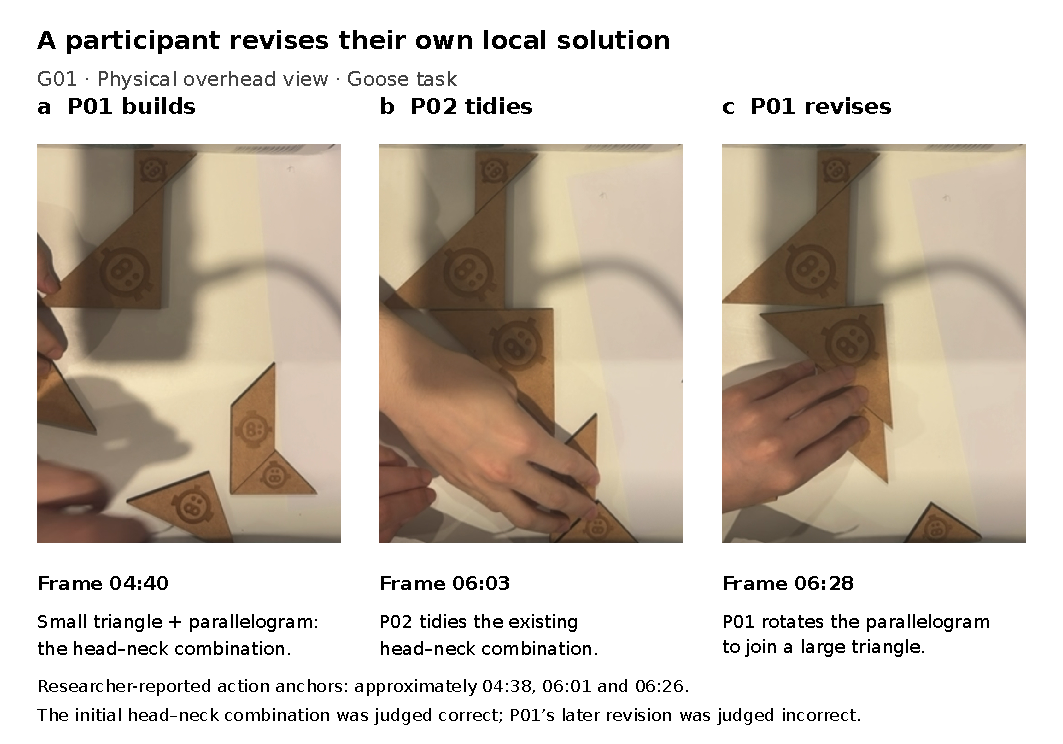
\includegraphics[width=\linewidth,height=96mm,keepaspectratio]{assets/figures/F4_self_revision.pdf}
\captionof{figure}[G01's physical-overhead goose task.]{G01's physical-overhead goose task. P01 builds the head and neck; P02 tidies the combination; P01 later rotates the parallelogram to join a large triangle. The researcher's video-review record judges the first local arrangement correct and the later revision incorrect. Frames at 04:40, 06:03 and 06:28 are close to reported action anchors at 04:38, 06:01 and 06:26. Crops remove call-interface identifiers and preserve the original projection. Hands occlude some edges; the middle still does not independently establish that P02 changed only alignment. [\hyperlink{src:D03}{D03}]}\label{fig:5-7}
\par\endgroup
\end{figureunit}



Here, the partner's intervention did not itself account for the loss of the correct head-and-neck arrangement. The reported sequence places P02's tidying before P01's explicit structural change. The event shows how a useful partial solution can be reopened by its original builder during a joint task.

G04's physical-direct task provides a second instance of a useful idea being reopened by its own builder. At approximately 05:30, P08 developed an approach that the researcher regarded as correct, then changed it again around 06:13. After this change, the researcher pointed out that the preceding approach had been correct. The task was eventually abandoned. This episode shows a useful construction being reopened by its own builder. [\hyperlink{src:D07}{D07}]

G03's first-person candle gives a different outcome for self-revision. P05 dismantled the small-triangle flame that P05 had made and repurposed its pieces for the base. Here, changing one's own work contributed to resolving the conflict between the two initial approaches. The contrast with G01 is instructive: self-revision can support progress or remove a correct part. Its consequence depends on the relationship between the revised part, the remaining pieces and the developing whole. [\hyperlink{src:D06}{D06}] The pose sequence in Figure~\ref{fig:5-5} adds a trace of one logged participant rearranging their own two-piece construction before the other participant handled those pieces.

In G05's first-person chair, the process notes describe P09 moving away from an almost-correct arrangement and changing the parallelogram's role, while P10 questioned the change. P10 later returned it to the backrest. This sequence joins self-revision to partner repair: the original builder's reconsideration did not simply end the attempt, because the partner later acted on the same part. The description of the earlier arrangement as almost correct comes from the process report. [\hyperlink{src:D10}{D10}]

Partners also changed each other's work. In G03's physical-direct horse task, P06 objected to P05's head construction and changed it while P05 continued with the body. In G01's physical-direct task, both partners repeatedly adjusted the same large triangle during a short disagreement around 01:36--01:40. These episodes show direct intervention in an existing local construction. They make the distinction between preservation, tidying and structural revision necessary when describing how a partner responded. [\hyperlink{src:D05}{D05}, \hyperlink{src:D02}{D02}]

G05 adds a related verbal sequence. P09 questioned the idea that the goose's body required large triangles and revised the idea while P10 gave no response during that interval. This is recorded as self-correction of a proposal. It complements the manipulation cases by showing that an apparent change in the pair's direction can originate in one person's reconsideration, even when both people are present. [\hyperlink{src:D09}{D09}]

G06's candle logs also show retention during reconstruction. No later pose change was recorded for the square after it settled at 59.79 active seconds, or for the new red large-triangle placement after 143.33 seconds, while other pieces continued to be manipulated. These retained placements and the surrounding rebuilding occurred within the same sequence. The statement concerns the recorded geometry at the logging resolution described in Section~\ref{sec:4-4}. [\hyperlink{src:D14}{D14}]

The finding concerns the trajectories of existing partial solutions: who develops them, who keeps them available, and who changes their structure. These trajectories reveal a form of coordination that a final picture alone would miss. A retained piece may carry earlier work into the next step, while a new manipulation can reopen a decision that had appeared settled. The video records establish the local interaction; where available, the pose logs make the change of operator and geometry directly traceable.


\section{Questionnaire perspectives on communication and control}\label{sec:5-4}

\begin{figureunit}{5-8}
The questionnaire adds a participant-level account of placement communication, progress awareness, piece control and joint solving (Figure~\ref{fig:5-8}). Ratings differed across these aspects. From first-person VR (R03) to shared overhead VR (R04), three participants rated explaining an intended placement more highly, eight gave the same rating and one gave a lower rating. Movement and rotation each received lower ratings from five participants, the same ratings from six and a higher rating from one. Communicating a placement and controlling a piece were therefore distinct aspects of the reported experience.

\par\begingroup
\centering
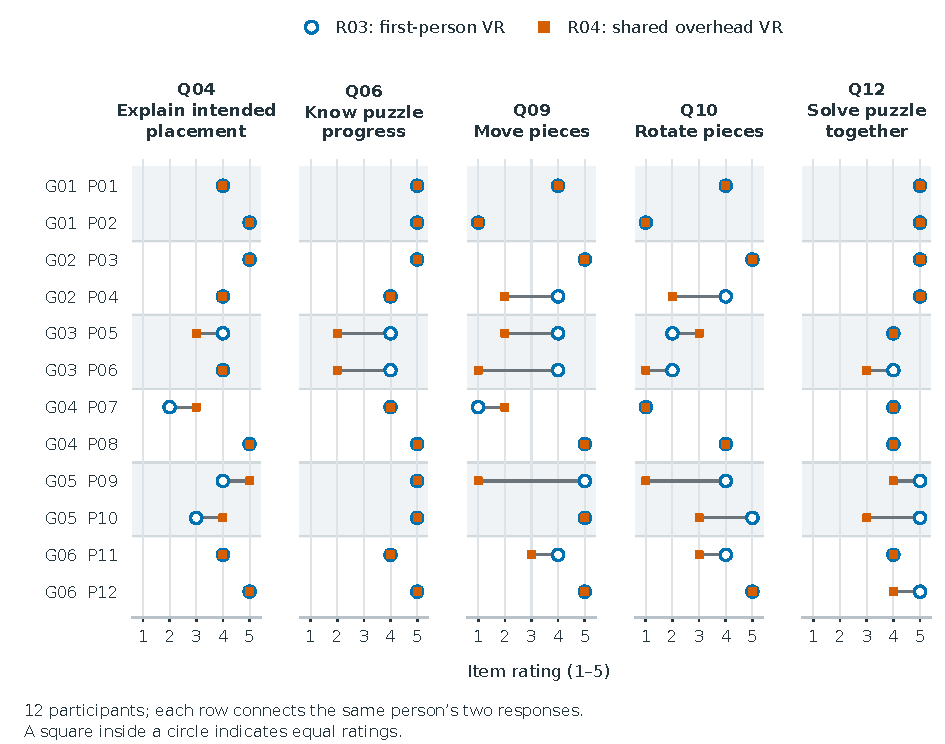
\includegraphics[width=\linewidth,height=120mm,keepaspectratio]{assets/figures/Figure5_8_VR_item_ratings.pdf}
\captionof{figure}[Paired ratings for five questionnaire items in first-person VR (R03) and shared overhead VR (R04).]{Paired ratings for five questionnaire items in first-person VR (R03) and shared overhead VR (R04). Each row is one participant; circles and squares show the two raw ratings, connected within that participant. A square inside a circle indicates equal ratings. All 12 participants have both responses for these items (24 VR questionnaires from the confirmed 48-response dataset). Q04 concerns explaining an intended placement, Q06 knowing puzzle progress, Q09 moving a piece to an intended location, Q10 rotating it to an intended orientation, and Q12 feeling that the puzzle was solved together. Ratings use the full 1--5 scale; no combined score is calculated. The rounds occurred in a fixed order with different target patterns. G01 used the earlier target presentation and G02--G06 the revised version. G02 ratings describe the original session; the relationship to the later recordings is explained in Section~\ref{sec:4-1}.}\label{fig:5-8}
\par\endgroup
\end{figureunit}

The differences are visible within dyads. In G05, both participants rated explaining a placement more highly in R04, while their ratings of solving together fell from 5 to 4 and from 5 to 3. P09 also rated moving pieces from 5 to 1 and rotating them from 4 to 1. In G04, both participants rated solving together at 4 in both rounds, although P07 rated rotation at 1 and P08 at 4. The questionnaire therefore supplements the action evidence by showing that a sense of working together can coexist with very different experiences of control. The comparisons describe sessions with a fixed condition order and different target patterns. G01 used the earlier target presentation; G02--G06 used the revised version.




\section{Connecting viewing conditions to the collaborative process}\label{sec:5-5}

The three findings connect through the evolving construction. Participants used the visible arrangement to decide where to work, which pieces to use and what to keep or revise. In G06, the initial division between body and top was followed by shared reconstruction around an apparently plausible candle. The partners completed the seven-piece arrangement and accepted it, while the later reconstruction confirmed the researcher's observation of a proportion problem. Viewing, work organisation and outcome judgment were therefore present within the same sequence.

The other cases show different paths through that relationship. G01 rejected a first-person candidate when a substitution failed to align. G05 continued working after a partner questioned the proportions. G03 reorganised overlapping local attempts by reallocating its small triangles. In the physical-overhead G01 case, a correct part was kept and tidied before its original builder changed it. These outcomes locate the contribution of an overhead view alongside the continuing work of interpreting, revising and coordinating a solution.

For this planar task, the overhead view's geometric advantage matters because shape and proportion are resources used throughout collaboration. The results support evaluating that view through the actual actions it accompanies: how participants establish a candidate, continue one another's work, notice a conflict and decide what to change. The action records also reveal why viewing the final arrangement alone provides an incomplete account of collaboration. The same ending can arise through different divisions of work, and a useful partial solution can be lost before the ending is reached.


\chapter{Discussion}\label{chap:6}

The study links the geometry available to partners with the actions through which they develop a construction. An arrangement can look plausible, become the basis for further work and be accepted even when its proportions differ from the target. Parts of that arrangement also have histories: one person builds them, another continues them, and either may later revise them. Following those histories connects the geometric value of an overhead view to the organisation of collaborative work.

\section{How the overhead view's geometric advantage enters collaboration}\label{sec:6-1}

Tangram makes local connections and the overall outline relevant to the same task. A piece must fit its neighbours, and the complete arrangement must match the target. Perspective projection from an oblique viewpoint changes the apparent lengths and angles of a planar construction. A perpendicular orthographic view preserves its relative shape and scale. This geometric property matters during collaboration because the developing shape is what partners use when they choose the next piece, assess a proposal and decide whether to continue changing the result.

G06 connects this property to an observed problem. Both partners helped rebuild the candle to include the unused medium triangle, and the seven-piece result was accepted by the pair and the researcher. The researcher later noticed that the accepted outline had a wider lower body than the target, and reconstruction confirmed that mismatch. The task account establishes that it was missed at the time. Their combination gives a concrete example of coordinated construction reaching an accepted result whose geometry still needed correction. [\hyperlink{src:D14}{D14}, \hyperlink{src:D16}{D16}]

The three first-person cases also show different responses to a plausible shape. G01 rejected a replacement when its edges failed to align. G05 continued after a partner questioned the chair's proportions. G06 accepted its final candle. The researcher's records identify this category in three of six first-person pairs and none of the six shared-overhead pairs. The comparison locates the problem within the implemented viewing conditions; the episodes explain how it entered the work. Agreement about an ending and the geometric validity of that ending are separate achievements.

Chen et al. compared a world-in-miniature interface and an interactive 2D map in collaborative searching and object manipulation \cite{chen2024}. Their discussion identifies a need to examine finer placement accuracy beyond placing objects within a designated work area. Tangram brings that issue into a planar construction where relative spans and edges determine whether a candidate matches the target. The present study also follows how partners form and revise the candidate, connecting spatial presentation with the sequence that produces the judged result.

The geometric advantage must be considered alongside control. In this prototype, the shared overhead image replaced the first-person scene while tracked controllers remained in the shared 3D workspace. G05 and G06 requested or provided help with difficult manipulations. Questionnaire responses likewise separated explaining a placement from moving or rotating a piece. A clear overall view can therefore coexist with difficulty carrying out the next local action. This combination makes the viewing arrangement and its manipulation mapping joint design concerns. [\hyperlink{src:D11}{D11}, \hyperlink{src:D15}{D15}]

\section{Expressing ideas through manipulation and taking turns to advance the task}\label{sec:6-2}

The partners' placements gave each other something concrete to inspect and continue. In G01's chicken, a demonstrated alternative for the back was followed by additions to the head. In G06's physical-overhead goose, P12 added a small triangle to an existing neck arrangement and P11 continued that addition with the medium triangle. Each action used what was already present and changed the possibilities for the next action. The sequence shows how a local construction can function as a proposal within the joint task. [\hyperlink{src:D01}{D01}, \hyperlink{src:D12}{D12}] These sequences develop a shared problem state through action, consistent with Roschelle and Teasley's account of proposals being presented and taken up through talk and manipulation \cite{roschelle1995}.

Dillenbourg describes how the distinction between cooperation and collaboration depends partly on the grain at which a division of labour is examined \cite{dillenbourg1999}. The Tangram cases make that grain visible at the level of parts and successive placements. A participant could develop a part independently for a short period, while the part remained dependent on the partner's preceding and subsequent work. The interpretation is therefore a changing organisation of connected actions: temporary division of work, continuation and joint revision can all occur within one attempt.

The G06 action trace provides a detailed example of that change. Initial work on the body and top developed into repeated manipulation of the same body pieces by both participants. Its paired pose sequence shows what those operations produced. G03 adds a different path: P05 brought two small triangles together, separated them and was followed by P06 operating on those pieces. Tracking operators together with configurations distinguishes a handover that continues an existing arrangement from one that changes the direction of construction. [\hyperlink{src:D14}{D14}, \hyperlink{src:D06}{D06}]

Workspace awareness includes following who is active and what is happening in the shared workspace \cite{gutwin2002}. The Tangram analysis follows the consequence of that activity for a developing arrangement. Yang et al. separated object interaction from meaningful changes of grouping in collaborative image organisation \cite{yang2022}. The same distinction matters here: a grab can adjust alignment, test a fit, expose a reference or change a piece's role. Reading the operation within its sequence explains its contribution to the task more clearly than the number of operations alone.

Irlitti et al. distinguished closely engaged collaboration, where one person manipulated objects while others discussed the task, from episodes where one person took over and others contributed little \cite{irlitti2024}. That distinction helps interpret the Tangram cases. A period of single-person manipulation can belong to joint work when it responds to the partner's preceding construction or provides a next step that the partner takes up. The evidence lies in those connections, so the analysis follows responses and changing arrangements alongside the distribution of control.

Manipulation can also help a participant develop an idea while acting. Kirsh and Maglio distinguish actions that advance a physical task from actions that make information easier to discover or evaluate \cite{kirsh1994}. Their account offers a way to understand why testing and rearranging pieces belongs within problem solving, even when a move is later reversed. In these cases, the observable evidence is the attempted relation and what follows it; the records support describing exploration without assigning a hidden cognitive purpose to every movement.

Rasch et al. studied undo in deliberately divided and collaborative VR tasks, then identified constantly changing collaboration arrangements as an issue for further work \cite{rasch2024}. The freely organised Tangram episodes show such changes within a task. The contribution lies in tracing how a local arrangement connects successive initiatives and revisions. This gives a concrete account of how work becomes joint at a fine scale, including moments when one participant is the only person manipulating a piece.

\section{Retaining a partner's partial arrangement and revising one's own}\label{sec:6-3}

A partial construction can remain available to the partner and later be reopened by its original builder. G01's correct goose head and neck survived the partner's tidying before its builder changed the relation into an incorrect one. G03's self-revision had a different consequence: dismantling a small-triangle arrangement made those pieces available for the developing solution. These cases show why revising a part and improving the whole are distinct. A change can resolve a conflict between parts or remove a useful local result. [\hyperlink{src:D03}{D03}, \hyperlink{src:D06}{D06}]

Retaining a construction also lets earlier work enter a later step. In G06's physical-overhead goose, successive additions developed from the existing neck and led to a correct outline with a different internal partition from the reference. The square and medium triangle occupied different regions, each paired with a small triangle. The outcome matters because the task allowed alternative internal solutions. Preservation supported a viable route through the problem even though that route differed from the reference construction. [\hyperlink{src:D12}{D12}]

The G06 interview gives one participant's interpretation of this behaviour: the partner's leaving placed pieces in position was taken as a sign of understanding. Yang et al. used a more specific criterion for respect in their image-organisation study: asking for permission before modifying another person's grouping \cite{yang2022}. These accounts concern different evidence. Here, retained geometry establishes that a construction remained available, while the interview explains what that action meant to a participant. Agreement or respect should be attributed through such contextual evidence. [\hyperlink{src:D13}{D13}]

An enacted alternative could prompt direct partner intervention. G01's chicken-back demonstration and G03's horse-head replacement occurred before the complete solution was established. In G05, the partner questioned the changed role of the parallelogram and later restored it to the backrest. These cases accompany the preservation and self-revision cases. The relevant comparison is whether an alternative was proposed or put into action in the recorded sequence, and what the partner did next. An absence of visible intervention provides no account of alternatives a participant might have considered privately. [\hyperlink{src:D01}{D01}, \hyperlink{src:D05}{D05}, \hyperlink{src:D10}{D10}]

G06's candle joins preservation to joint rebuilding. The square and the later red large-triangle placement persisted in the pose record while both participants continued to adjust other pieces. This establishes a stable part of the evolving construction around which further action occurred. The eventual result still had the measured proportion mismatch. Examining both histories explains how coordinated continuation and an incorrect outcome can coexist: the pair advanced a shared arrangement, while some of its geometric relations survived the ongoing changes. [\hyperlink{src:D14}{D14}, \hyperlink{src:D16}{D16}]

\section{Design implications for shared-overhead VR}\label{sec:6-4}

Shared-overhead VR should make overall geometric relations easy to inspect during construction. G06's request for another viewpoint shows a participant treating viewing as a resource for resolving the task. A design with accessible switching could let partners move between local manipulation and inspection of the whole arrangement. Piece identities, the target and orientation cues should remain recognisable across that transition so that the construction can be continued. Its value should be evaluated through the checking and subsequent actions that the view supports. [\hyperlink{src:D14}{D14}]

Manipulation needs comparable attention. Assistance in G05 and G06 shows a practical route through a blocked action: another participant carries out an adjustment, then work continues. Interfaces should make a piece's current control state clear and allow brief transfers without forcing a permanent director--operator arrangement. The relevant outcome is whether partners can complete the requested adjustment and resume their work. The prototype's direction mapping and reach difficulties should be addressed alongside visual clarity, because both affect who can carry out an available next step. [\hyperlink{src:D11}{D11}, \hyperlink{src:D15}{D15}]

Construction history offers a further way to support revision. The cases suggest retaining access to earlier local arrangements so that partners can compare or recover a useful relation after changing it. Rasch et al. found that the scope of undo in multi-user VR affects both recovery and disturbance to a partner's work \cite{rasch2024}. Their results motivate careful choice of what a restoration changes. For Tangram, an inspectable earlier state could support discussion before a shared arrangement is restored; this proposal remains to be evaluated in use.

Evaluation should connect these features to episodes of work. For a view change, the question is which relation becomes inspectable and what the partners do with it. For assistance, it is whether control passes successfully and the blocked placement is completed. For history, it is which earlier arrangement is recovered and how later additions are affected. These questions preserve the connection between interface behaviour, changing geometry and the partners' next actions that made the present cases informative.

\section{Study scope and further evaluation}\label{sec:6-5}

The findings describe six familiar pairs working through four conditions in a fixed order. Target patterns and familiarisation varied; G01's first recording used an earlier target presentation, while the recorded G02--G06 sessions used the revised version. The three-of-six versus zero-of-six comparison concerns the defined near-complete shape problem in the researcher's records. It is separate from a uniform geometric inspection of every ending and from an estimate of viewpoint's independent effect. A subsequent comparison can stabilise the controls and target presentation, then balance patterns and order.

The analysis combines sources with different strengths. Researcher process reports locate proposals, responses and visible actions. Logs identify accepted control and recorded geometry; selected reconstructions check shape problems that the researcher identified during review. Interview paraphrases provide participants' retrospective meanings. Missing audio limits the attribution of some spoken turns, while the retained source references keep those boundaries visible. The G06 reconstruction applies the existing outline requirement, preserving both the original acceptance and the subsequent correction.

The selected revision cases establish sequences, including instances of self-revision and direct partner intervention. They support comparing how a partial solution was treated and what happened to it. Establishing their relative frequency would require consistent episode definitions applied across all recorded processes. The current contribution is the linked account: who first formed an arrangement, how it remained available, who changed it and how its geometry developed. This level of analysis makes useful local work and its possible loss visible within the broader task.


The findings give a more specific answer to the initial expectations. The overview's value is visible in the planar relationships available for checking a construction, while the overhead cases also show the importance of usable control and local help. The construction sequences explain how partners temporarily divide, continue and revise work across conditions. They leave open the earlier question of whether viewpoint changes personal agency or ownership: the present analysis traces how partial arrangements are treated, while that broader experience was not measured as a separate construct. [\hyperlink{src:D32}{D32}, \hyperlink{src:D31}{D31}]

\chapter{Conclusion}\label{chap:7}

Six pairs solved Tangram together in shared overhead VR and related physical and first-person conditions. This thesis followed how they judged shapes, expressed ideas through manipulation and responded to existing constructions.

The first finding concerns the geometric problems encountered during construction. The researcher's records identified near-complete shape problems in three of six first-person VR pairs and none of the six shared-overhead VR pairs. G06's candle showed why an accepted ending deserved closer examination: all seven pieces had been incorporated, yet the overall outline still differed from the target. This case connects the presentation of planar geometry to the pair's practical judgment of its result.

The second and third findings explain how constructions developed. Participants made local ideas visible through placements that their partners could extend or change. Work moved between separate parts, assistance and shared reconstruction. Partners also retained or continued partial arrangements that their original builders later revised. Self-revision could help the task progress or remove a correct part, while concrete alternatives could prompt direct partner intervention.

The project developed from eight proposed combinations and a separate construction task into Tangram across four conditions, with participants organising their collaboration freely. It delivered a shared overhead prototype and a six-pair corpus. Formal rounds used a fixed viewpoint. Target presentation changed between G01's initial recording and the revised sessions for G02--G06. These development decisions and the fixed condition order define the comparison presented here.

These processes support an inspectable overview, usable manipulation and brief assistance. Further evaluation can test viewpoint switching and access to earlier configurations with balanced tasks and stable controls.


\clearpage
\phantomsection\addcontentsline{toc}{chapter}{Bibliography}
\begingroup\singlespacing\small
\bibliographystyle{unsrt}
\bibliography{references}
\endgroup
\appendix
\chapter{Evidence and source navigation}\label{chap:A}

The D numbers below identify the study records and project documents used in this thesis. Clicking a D reference in the text opens the corresponding entry here. The Files links open the repository source catalogue, which records availability and links to public materials. Published research is listed separately in the bibliography. Original recordings, signed consent forms and private correspondence are retained separately; access to restricted records requires an authorised arrangement.

Stable participant numbers P01--P12 are used across the physical and VR conditions. Original recording-position labels have been mapped using the researcher's clarification, and selected software-endpoint mappings have been checked against visible grabs.

Table~\ref{tab:A-3} records the six-dyad comparison for the defined near-target configuration category, including the evidence for each pair. [\hyperlink{src:D27}{D27}]

\begingroup
\setstretch{1}
\fontsize{10}{12.3}\selectfont
\setlength{\tabcolsep}{2.2pt}
\renewcommand{\arraystretch}{1.18}
\begin{longtable}{@{}>{\raggedright\arraybackslash}p{16.343mm}>{\raggedright\arraybackslash}p{34.368mm}>{\raggedright\arraybackslash}p{34.368mm}>{\raggedright\arraybackslash}p{34.368mm}>{\raggedright\arraybackslash}p{34.368mm}@{}}
\caption[Process-report navigation by group and research condition.]{Process-report navigation by group and research condition.}\label{tab:A-1}\\
\toprule
\textbf{Group} & \textbf{R01} & \textbf{R02} & \textbf{R03} & \textbf{R04} \\
\midrule
\endfirsthead
\multicolumn{5}{l}{\small\itshape Table \thetable{} (continued)}\\
\toprule
\textbf{Group} & \textbf{R01} & \textbf{R02} & \textbf{R03} & \textbf{R04} \\
\midrule
\endhead
\midrule
\multicolumn{5}{r}{\small Continued on next page}\\
\endfoot
\bottomrule
\endlastfoot
G01 & \hyperlink{src:D01}{D01} & \hyperlink{src:D03}{D03} & \hyperlink{src:D48}{D48};\hyperlink{src:D04}{D04} & \hyperlink{src:D49}{D49};\hyperlink{src:D51}{D51} \\
\addlinespace[3pt]
G02 & \hyperlink{src:D52}{D52} & \hyperlink{src:D53}{D53};\hyperlink{src:D54}{D54} & \hyperlink{src:D55}{D55} & \hyperlink{src:D56}{D56} \\
\addlinespace[3pt]
G03 & \hyperlink{src:D05}{D05} & \hyperlink{src:D57}{D57} & \hyperlink{src:D06}{D06} & \hyperlink{src:D58}{D58};\hyperlink{src:D59}{D59} \\
\addlinespace[3pt]
G04 & \hyperlink{src:D07}{D07} & \hyperlink{src:D60}{D60} & \hyperlink{src:D08}{D08} & \hyperlink{src:D61}{D61} \\
\addlinespace[3pt]
G05 & \hyperlink{src:D09}{D09} & \hyperlink{src:D62}{D62}; \hyperlink{src:D64}{D64} & \hyperlink{src:D10}{D10} & \hyperlink{src:D11}{D11}; \hyperlink{src:D65}{D65} \\
\addlinespace[3pt]
G06 & \hyperlink{src:D63}{D63} & \hyperlink{src:D12}{D12} & \hyperlink{src:D14}{D14} & \hyperlink{src:D15}{D15} \\
\end{longtable}
\endgroup

\begingroup
\setstretch{1}
\fontsize{10}{12.3}\selectfont
\setlength{\tabcolsep}{3pt}
\renewcommand{\arraystretch}{1.16}
\begin{longtable}{@{}p{14mm}>{\raggedright\arraybackslash}p{140mm}@{}}
\caption[Data and project sources.]{Data and project sources. The D numbers identify study records and project documents; numbered bibliography entries identify published research. Files links open the repository source catalogue and access information.}\label{tab:A-2}\\
\toprule
\textbf{Source} & \textbf{Record and file link}\\
\midrule
\endfirsthead
\multicolumn{2}{l}{\small\itshape Table \thetable{} (continued)}\\
\toprule
\textbf{Source} & \textbf{Record and file link}\\
\midrule
\endhead
\midrule
\multicolumn{2}{r}{\small Continued on next page}\\
\endfoot
\bottomrule
\endlastfoot
\hypertarget{src:D01}{}\label{src:D01}D01 & G01 physical-direct chicken: local alternative enacted by P02, followed by head construction proposed by P01. \href{https://github.com/YiyangQin-UQ/REIT7841/blob/main/thesis/v1.1/materials/README.md\#d01}{\textit{Files}} \\
\hypertarget{src:D02}{}\label{src:D02}D02 & G01 physical-direct task: repeated adjustment of the same large triangle. \href{https://github.com/YiyangQin-UQ/REIT7841/blob/main/thesis/v1.1/materials/README.md\#d02}{\textit{Files}} \\
\hypertarget{src:D03}{}\label{src:D03}D03 & G01 physical-overhead goose: head/neck construction, tidying and self-revision; latest researcher correction. \href{https://github.com/YiyangQin-UQ/REIT7841/blob/main/thesis/v1.1/materials/README.md\#d03}{\textit{Files}} \\
\hypertarget{src:D04}{}\label{src:D04}D04 & G01 first-person chair; combined two-endpoint account, v049 revision. \href{https://github.com/YiyangQin-UQ/REIT7841/blob/main/thesis/v1.1/materials/README.md\#d04}{\textit{Files}} \\
\hypertarget{src:D05}{}\label{src:D05}D05 & G03 physical-direct horse: P06 changes the head while P05 continues the body. \href{https://github.com/YiyangQin-UQ/REIT7841/blob/main/thesis/v1.1/materials/README.md\#d05}{\textit{Files}} \\
\hypertarget{src:D06}{}\label{src:D06}D06 & G03 first-person candle: different flame attempts, common-side move and small-triangle reassignment; original action/pose log. \href{https://github.com/YiyangQin-UQ/REIT7841/blob/main/thesis/v1.1/materials/README.md\#d06}{\textit{Files}} \\
\hypertarget{src:D07}{}\label{src:D07}D07 & G04 physical-direct goose: useful approach revisited, followed by researcher feedback. \href{https://github.com/YiyangQin-UQ/REIT7841/blob/main/thesis/v1.1/materials/README.md\#d07}{\textit{Files}} \\
\hypertarget{src:D08}{}\label{src:D08}D08 & G04 first-person candle: structure explanation and complementary placements; original log. \href{https://github.com/YiyangQin-UQ/REIT7841/blob/main/thesis/v1.1/materials/README.md\#d08}{\textit{Files}} \\
\hypertarget{src:D09}{}\label{src:D09}D09 & G05 physical-direct goose: P09's verbal self-correction. \href{https://github.com/YiyangQin-UQ/REIT7841/blob/main/thesis/v1.1/materials/README.md\#d09}{\textit{Files}} \\
\hypertarget{src:D10}{}\label{src:D10}D10 & G05 first-person chair: proportion problem, self-revision and partner repair. \href{https://github.com/YiyangQin-UQ/REIT7841/blob/main/thesis/v1.1/materials/README.md\#d10}{\textit{Files}} \\
\hypertarget{src:D11}{}\label{src:D11}D11 & G05 shared-overhead task: suggestions, manipulation and local assistance. \href{https://github.com/YiyangQin-UQ/REIT7841/blob/main/thesis/v1.1/materials/README.md\#d11}{\textit{Files}} \\
\hypertarget{src:D12}{}\label{src:D12}D12 & G06 physical-overhead goose: successive additions and a correct alternative internal partition; v072 image supplement. \href{https://github.com/YiyangQin-UQ/REIT7841/blob/main/thesis/v1.1/materials/README.md\#d12}{\textit{Files}} \\
\hypertarget{src:D13}{}\label{src:D13}D13 & G06 group interview, original interview.docx paragraph 11; paraphrases with unresolved within-pair speaker attribution. \href{https://github.com/YiyangQin-UQ/REIT7841/blob/main/thesis/v1.1/materials/README.md\#d13}{\textit{Files}} \\
\hypertarget{src:D14}{}\label{src:D14}D14 & G06 first-person candle: process report, original video and original action/pose log. \href{https://github.com/YiyangQin-UQ/REIT7841/blob/main/thesis/v1.1/materials/README.md\#d14}{\textit{Files}} \\
\hypertarget{src:D15}{}\label{src:D15}D15 & G06 shared-overhead task: valid restarted round and local assistance. \href{https://github.com/YiyangQin-UQ/REIT7841/blob/main/thesis/v1.1/materials/README.md\#d15}{\textit{Files}} \\
\hypertarget{src:D16}{}\label{src:D16}D16 & G06 geometry correction and current recomputation from saved mesh plus recorded poses. \href{https://github.com/YiyangQin-UQ/REIT7841/blob/main/thesis/v1.1/materials/README.md\#d16}{\textit{Files}} \\
\hypertarget{src:D17}{}\label{src:D17}D17 & Completed source-report queue and designation of one formal process per dyad and condition. \href{https://github.com/YiyangQin-UQ/REIT7841/blob/main/thesis/v1.1/materials/README.md\#d17}{\textit{Files}} \\
\hypertarget{src:D18}{}\label{src:D18}D18 & Researcher clarifications about familiar partners, prior experience, familiarisation and on-site judgment. \href{https://github.com/YiyangQin-UQ/REIT7841/blob/main/thesis/v1.1/materials/README.md\#d18}{\textit{Files}} \\
\hypertarget{src:D19}{}\label{src:D19}D19 & Recording coverage and the absence of usable R02 audio. \href{https://github.com/YiyangQin-UQ/REIT7841/blob/main/thesis/v1.1/materials/README.md\#d19}{\textit{Files}} \\
\hypertarget{src:D20}{}\label{src:D20}D20 & Confirmed questionnaire table, confirmation provenance and original Chinese item wording. \href{https://github.com/YiyangQin-UQ/REIT7841/blob/main/thesis/v1.1/materials/README.md\#d20}{\textit{Files}} \\
\hypertarget{src:D21}{}\label{src:D21}D21 & Selected event/pose traces and cross-source case records used for the figures and action sequences. \href{https://github.com/YiyangQin-UQ/REIT7841/blob/main/thesis/v1.1/materials/README.md\#d21}{\textit{Files}} \\
\hypertarget{src:D22}{}\label{src:D22}D22 & Retained consent forms and the supervisor's educational-use correspondence. \href{https://github.com/YiyangQin-UQ/REIT7841/blob/main/thesis/v1.1/materials/README.md\#d22}{\textit{Files}} \\
\hypertarget{src:D23}{}\label{src:D23}D23 & Documented assistance and figure-generation records for the present drafting process. \href{https://github.com/YiyangQin-UQ/REIT7841/blob/main/thesis/v1.1/materials/README.md\#d23}{\textit{Files}} \\
\hypertarget{src:D24}{}\label{src:D24}D24 & Implemented three-smartphone Discord apparatus and two-headset VR arrangement, with viewing and control mappings. \href{https://github.com/YiyangQin-UQ/REIT7841/blob/main/thesis/v1.1/materials/README.md\#d24}{\textit{Files}} \\
\hypertarget{src:D25}{}\label{src:D25}D25 & Collection-period logging definitions, original protocol metadata and software-attempt boundaries. \href{https://github.com/YiyangQin-UQ/REIT7841/blob/main/thesis/v1.1/materials/README.md\#d25}{\textit{Files}} \\
\hypertarget{src:D26}{}\label{src:D26}D26 & Last-known-pose reconstruction, post-release records, retained source rows and chord/span geometry definition. \href{https://github.com/YiyangQin-UQ/REIT7841/blob/main/thesis/v1.1/materials/README.md\#d26}{\textit{Files}} \\
\hypertarget{src:D27}{}\label{src:D27}D27 & Later researcher confirmation of the same near-target configuration category across the six R03/R04 records; G02 is included with all six pairs. \href{https://github.com/YiyangQin-UQ/REIT7841/blob/main/thesis/v1.1/materials/README.md\#d27}{\textit{Files}} \\
\hypertarget{src:D28}{}\label{src:D28}D28 & Original supervisor project description: collaborative behaviour, communication, coordination and workspace awareness in third-person VR. \href{https://github.com/YiyangQin-UQ/REIT7841/blob/main/thesis/v1.1/materials/README.md\#d28}{\textit{Files}} \\
\hypertarget{src:D29}{}\label{src:D29}D29 & Early physical Tangram study plan (StudyTestPlan\_Iteration\_1); a planning record preceding the implemented study. \href{https://github.com/YiyangQin-UQ/REIT7841/blob/main/thesis/v1.1/materials/README.md\#d29}{\textit{Files}} \\
\hypertarget{src:D30}{}\label{src:D30}D30 & Early thesis project roadmap, covering the planned progression from physical collaboration to a VR prototype. \href{https://github.com/YiyangQin-UQ/REIT7841/blob/main/thesis/v1.1/materials/README.md\#d30}{\textit{Files}} \\
\hypertarget{src:D31}{}\label{src:D31}D31 & August thesis plan, including the shared spatial representation rationale and proposed physical and VR tasks. \href{https://github.com/YiyangQin-UQ/REIT7841/blob/main/thesis/v1.1/materials/README.md\#d31}{\textit{Files}} \\
\hypertarget{src:D32}{}\label{src:D32}D32 & Student email of 19 August 2026 discussing the thesis plan and how to examine collaboration beyond spatial overlap or activity counts. \href{https://github.com/YiyangQin-UQ/REIT7841/blob/main/thesis/v1.1/materials/README.md\#d32}{\textit{Files}} \\
\hypertarget{src:D33}{}\label{src:D33}D33 & Supervisor response of 20 August 2026 on task comparability and the possibility of both separate and joint work. \href{https://github.com/YiyangQin-UQ/REIT7841/blob/main/thesis/v1.1/materials/README.md\#d33}{\textit{Files}} \\
\hypertarget{src:D34}{}\label{src:D34}D34 & Supervisor meeting transcript indexed to 22 April 2026; discussion of the research aim and prototype development. \href{https://github.com/YiyangQin-UQ/REIT7841/blob/main/thesis/v1.1/materials/README.md\#d34}{\textit{Files}} \\
\hypertarget{src:D35}{}\label{src:D35}D35 & Supervisor meeting transcript indexed to 12 June 2026; discussion of separate work and joint responsibility within a collaborative task. \href{https://github.com/YiyangQin-UQ/REIT7841/blob/main/thesis/v1.1/materials/README.md\#d35}{\textit{Files}} \\
\hypertarget{src:D36}{}\label{src:D36}D36 & Supervisor meeting transcript indexed to 1 September 2026; comparison of task options and selection of a common Tangram task family. \href{https://github.com/YiyangQin-UQ/REIT7841/blob/main/thesis/v1.1/materials/README.md\#d36}{\textit{Files}} \\
\hypertarget{src:D37}{}\label{src:D37}D37 & Intermediate eight-condition test plan, including assigned-role and free-collaboration variants; retained as design history. \href{https://github.com/YiyangQin-UQ/REIT7841/blob/main/thesis/v1.1/materials/README.md\#d37}{\textit{Files}} \\
\hypertarget{src:D38}{}\label{src:D38}D38 & Final Chinese researcher procedure manual, version 3, used to document the study procedure. \href{https://github.com/YiyangQin-UQ/REIT7841/blob/main/thesis/v1.1/materials/README.md\#d38}{\textit{Files}} \\
\hypertarget{src:D39}{}\label{src:D39}D39 & Submitted conference paper, particularly its method description of the physical and VR configurations. \href{https://github.com/YiyangQin-UQ/REIT7841/blob/main/thesis/v1.1/materials/README.md\#d39}{\textit{Files}} \\
\hypertarget{src:D40}{}\label{src:D40}D40 & Researcher clarification of formal-round designation and the implemented overhead VR display and control arrangement. \href{https://github.com/YiyangQin-UQ/REIT7841/blob/main/thesis/v1.1/materials/README.md\#d40}{\textit{Files}} \\
\hypertarget{src:D41}{}\label{src:D41}D41 & Implementation check of the world-fixed overhead camera, head-following screen and relationship between viewing and controller directions. \href{https://github.com/YiyangQin-UQ/REIT7841/blob/main/thesis/v1.1/materials/README.md\#d41}{\textit{Files}} \\
\hypertarget{src:D42}{}\label{src:D42}D42 & Cross-group record of actual attempts, practice, restarts and implementation differences. \href{https://github.com/YiyangQin-UQ/REIT7841/blob/main/thesis/v1.1/materials/README.md\#d42}{\textit{Files}} \\
\hypertarget{src:D43}{}\label{src:D43}D43 & Cross-group record of target-presentation versions, distinguishing earlier individual targets from the later shared target. \href{https://github.com/YiyangQin-UQ/REIT7841/blob/main/thesis/v1.1/materials/README.md\#d43}{\textit{Files}} \\
\hypertarget{src:D44}{}\label{src:D44}D44 & Documented analysis procedure: within-dyad process comparison, source distinctions and interpretation of questionnaire and action records. \href{https://github.com/YiyangQin-UQ/REIT7841/blob/main/thesis/v1.1/materials/README.md\#d44}{\textit{Files}} \\
\hypertarget{src:D45}{}\label{src:D45}D45 & Researcher clarification separating G04's familiarisation attempts from the formal overhead swimmer task. \href{https://github.com/YiyangQin-UQ/REIT7841/blob/main/thesis/v1.1/materials/README.md\#d45}{\textit{Files}} \\
\hypertarget{src:D46}{}\label{src:D46}D46 & Researcher clarification that participant position changes were self-initiated, with researcher interventions recorded separately. \href{https://github.com/YiyangQin-UQ/REIT7841/blob/main/thesis/v1.1/materials/README.md\#d46}{\textit{Files}} \\
\hypertarget{src:D47}{}\label{src:D47}D47 & Four-condition table and implementation description linking R01--R04 to the physical and virtual viewing arrangements. \href{https://github.com/YiyangQin-UQ/REIT7841/blob/main/thesis/v1.1/materials/README.md\#d47}{\textit{Files}} \\
\hypertarget{src:D48}{}\label{src:D48}D48 & G01 first-person VR chair: researcher report from one recording endpoint, read with the combined \hyperlink{src:D04}{D04} account. \href{https://github.com/YiyangQin-UQ/REIT7841/blob/main/thesis/v1.1/materials/README.md\#d48}{\textit{Files}} \\
\hypertarget{src:D49}{}\label{src:D49}D49 & G01 shared-overhead VR person: endpoint-specific speech and action reports, including the clarification of recording coverage. \href{https://github.com/YiyangQin-UQ/REIT7841/blob/main/thesis/v1.1/materials/README.md\#d49}{\textit{Files}} \\
\hypertarget{src:D50}{}\label{src:D50}D50 & G01 candle practice: orientation negotiation and pre-formal-task exposure; excluded from the four formal research conditions. \href{https://github.com/YiyangQin-UQ/REIT7841/blob/main/thesis/v1.1/materials/README.md\#d50}{\textit{Files}} \\
\hypertarget{src:D51}{}\label{src:D51}D51 & G01 shared-overhead VR person: disagreement about the base, local agreement and later retention of the proposed solution. \href{https://github.com/YiyangQin-UQ/REIT7841/blob/main/thesis/v1.1/materials/README.md\#d51}{\textit{Files}} \\
\hypertarget{src:D52}{}\label{src:D52}D52 & G02 physical-direct task: researcher process report of suggestions and subsequent manipulation. \href{https://github.com/YiyangQin-UQ/REIT7841/blob/main/thesis/v1.1/materials/README.md\#d52}{\textit{Files}} \\
\hypertarget{src:D53}{}\label{src:D53}D53 & G02 physical-overhead bull: researcher process report and clarification of the horn arrangement and subsequent tidying. \href{https://github.com/YiyangQin-UQ/REIT7841/blob/main/thesis/v1.1/materials/README.md\#d53}{\textit{Files}} \\
\hypertarget{src:D54}{}\label{src:D54}D54 & G02 physical-overhead bull: supplementary clarification of the target's horn outline and the interpretation of the local construction. \href{https://github.com/YiyangQin-UQ/REIT7841/blob/main/thesis/v1.1/materials/README.md\#d54}{\textit{Files}} \\
\hypertarget{src:D55}{}\label{src:D55}D55 & G02 first-person VR person task: base negotiation and work on different parts; later recording with a new target. \href{https://github.com/YiyangQin-UQ/REIT7841/blob/main/thesis/v1.1/materials/README.md\#d55}{\textit{Files}} \\
\hypertarget{src:D56}{}\label{src:D56}D56 & G02 overhead VR boat task: same-side position adjustment and continued construction; later recording with a new target. \href{https://github.com/YiyangQin-UQ/REIT7841/blob/main/thesis/v1.1/materials/README.md\#d56}{\textit{Files}} \\
\hypertarget{src:D57}{}\label{src:D57}D57 & G03 physical-overhead rabbit: local requests, action continuation and revision of the body. \href{https://github.com/YiyangQin-UQ/REIT7841/blob/main/thesis/v1.1/materials/README.md\#d57}{\textit{Files}} \\
\hypertarget{src:D58}{}\label{src:D58}D58 & G03 shared-overhead VR chair: two-endpoint process report of specific instructions, partner actions, manipulation difficulty and completion. \href{https://github.com/YiyangQin-UQ/REIT7841/blob/main/thesis/v1.1/materials/README.md\#d58}{\textit{Files}} \\
\hypertarget{src:D59}{}\label{src:D59}D59 & G03 shared-overhead VR chair: clarification of the researcher's second structural hint about which pieces formed the base and backrest. \href{https://github.com/YiyangQin-UQ/REIT7841/blob/main/thesis/v1.1/materials/README.md\#d59}{\textit{Files}} \\
\hypertarget{src:D60}{}\label{src:D60}D60 & G04 physical-overhead bull: revision of the horn candidate and the partner's independent placement of a piece. \href{https://github.com/YiyangQin-UQ/REIT7841/blob/main/thesis/v1.1/materials/README.md\#d60}{\textit{Files}} \\
\hypertarget{src:D61}{}\label{src:D61}D61 & G04 shared-overhead VR swimmer: grabbing difficulty and task continuation, documented from the recording that covers the formal round. \href{https://github.com/YiyangQin-UQ/REIT7841/blob/main/thesis/v1.1/materials/README.md\#d61}{\textit{Files}} \\
\hypertarget{src:D62}{}\label{src:D62}D62 & G05 physical-overhead rabbit: continued work on local parts and the distinction between construction and checking after completion. \href{https://github.com/YiyangQin-UQ/REIT7841/blob/main/thesis/v1.1/materials/README.md\#d62}{\textit{Files}} \\
\hypertarget{src:D63}{}\label{src:D63}D63 & G06 physical-direct horse: local attempts, changed piece placements and continuation following a partner's suggestion. \href{https://github.com/YiyangQin-UQ/REIT7841/blob/main/thesis/v1.1/materials/README.md\#d63}{\textit{Files}} \\
\hypertarget{src:D64}{}\label{src:D64}D64 & Earlier researcher notes for G05's physical-overhead rabbit, retained alongside the later \hyperlink{src:D62}{D62} clarification. \href{https://github.com/YiyangQin-UQ/REIT7841/blob/main/thesis/v1.1/materials/README.md\#d64}{\textit{Files}} \\
\hypertarget{src:D65}{}\label{src:D65}D65 & Earlier researcher notes for G05's shared-overhead VR person, covering suggestions, manipulation and requests for local assistance. \href{https://github.com/YiyangQin-UQ/REIT7841/blob/main/thesis/v1.1/materials/README.md\#d65}{\textit{Files}} \\
\hypertarget{src:D66}{}\label{src:D66}D66 & G04 endpoint video containing first-person VR and earlier overhead familiarisation; the surviving segment does not cover the formal swimmer round. \href{https://github.com/YiyangQin-UQ/REIT7841/blob/main/thesis/v1.1/materials/README.md\#d66}{\textit{Files}} \\
\hypertarget{src:D67}{}\label{src:D67}D67 & G04 partner-endpoint video covering the formal shared-overhead swimmer round, used for the \hyperlink{src:D61}{D61} process account. \href{https://github.com/YiyangQin-UQ/REIT7841/blob/main/thesis/v1.1/materials/README.md\#d67}{\textit{Files}} \\
\hypertarget{src:D68}{}\label{src:D68}D68 & Supervisor discussion indexed to 13 October 2026: analysing interactions and revisiting hypotheses. \href{https://github.com/YiyangQin-UQ/REIT7841/blob/main/thesis/v1.1/materials/README.md\#d68}{\textit{Files}} \\
\hypertarget{src:D69}{}\label{src:D69}D69 & Researcher original planning message: remove prescribed roles after trying the study; retain freely negotiated work. \href{https://github.com/YiyangQin-UQ/REIT7841/blob/main/thesis/v1.1/materials/README.md\#d69}{\textit{Files}} \\
\hypertarget{src:D70}{}\label{src:D70}D70 & Researcher original message on qualitative/quantitative records, interviews and explanations for each method. \href{https://github.com/YiyangQin-UQ/REIT7841/blob/main/thesis/v1.1/materials/README.md\#d70}{\textit{Files}} \\
\hypertarget{src:D71}{}\label{src:D71}D71 & Archived thesis-planning conversation, including the proposed four-layer data-collection rationale. \href{https://github.com/YiyangQin-UQ/REIT7841/blob/main/thesis/v1.1/materials/README.md\#d71}{\textit{Files}} \\
\hypertarget{src:D72}{}\label{src:D72}D72 & Original proposal: method selection and anticipated outcomes. \href{https://github.com/YiyangQin-UQ/REIT7841/blob/main/thesis/v1.1/materials/README.md\#d72}{\textit{Files}} \\
\hypertarget{src:D73}{}\label{src:D73}D73 & Data-collection rationale and Unity logging plan V3. \href{https://github.com/YiyangQin-UQ/REIT7841/blob/main/thesis/v1.1/materials/README.md\#d73}{\textit{Files}} \\
\hypertarget{src:D74}{}\label{src:D74}D74 & Researcher clarification of participant identities, revised prototype experience, G02 targets and the origin of the focal observations, 2 November 2026. \href{https://github.com/YiyangQin-UQ/REIT7841/blob/main/thesis/v1.1/materials/README.md\#d74}{\textit{Files}} \\
\end{longtable}
\endgroup

\begingroup
\setstretch{1}
\fontsize{9.5}{11.685}\selectfont
\setlength{\tabcolsep}{2.2pt}
\renewcommand{\arraystretch}{1.18}
\begin{longtable}{@{}>{\raggedright\arraybackslash}p{12.623mm}>{\raggedright\arraybackslash}p{45.637mm}>{\raggedright\arraybackslash}p{38.840mm}>{\raggedright\arraybackslash}p{58.260mm}@{}}
\caption[Process judgments for the same class of near-target configuration problem across R03 and R04.]{Process judgments for the same class of near-target configuration problem across R03 and R04.}\label{tab:A-3}\\
\toprule
\textbf{Dyad} & \textbf{R03: first-person VR} & \textbf{R04: shared-overhead VR} & \textbf{Evidence and qualification} \\
\midrule
\endfirsthead
\multicolumn{4}{l}{\small\itshape Table \thetable{} (continued)}\\
\toprule
\textbf{Dyad} & \textbf{R03: first-person VR} & \textbf{R04: shared-overhead VR} & \textbf{Evidence and qualification} \\
\midrule
\endhead
\midrule
\multicolumn{4}{r}{\small Continued on next page}\\
\endfoot
\bottomrule
\endlastfoot
G01 & Reported: chair/H candidate with an unused medium triangle; the attempted replacement did not fit. & Not reported for the specified category. & \hyperlink{src:D04}{D04}, \href{https://github.com/YiyangQin-UQ/REIT7841/blob/main/thesis/v1.1/materials/README.md\#d04}{V20} about 07:30--08:11; \hyperlink{src:D51}{D51}. The problem was noticed during the task. \\
\addlinespace[3pt]
G02 & Not reported for the specified category. & Not reported for the specified category. & \hyperlink{src:D55}{D55}/\hyperlink{src:D56}{D56} cover the person and boat tasks recorded later using new target patterns. Both conditions are included in the six-pair analysis. \\
\addlinespace[3pt]
G03 & Not reported for the specified category; candle record used as a geometric comparison. & Not reported for the specified category; chair task included structural hints. & \hyperlink{src:D06}{D06}; \hyperlink{src:D58}{D58}/\hyperlink{src:D59}{D59}. Difficulty placing a remaining part alone does not satisfy the near-target-whole criterion. \\
\addlinespace[3pt]
G04 & Not reported for the specified category; candle record used as a geometric comparison. & Not reported for the specified category; swimmer record includes grasping difficulty. & \hyperlink{src:D08}{D08}/\hyperlink{src:D61}{D61}. Control difficulty is distinguished from a near-target configuration mismatch. \\
\addlinespace[3pt]
G05 & Reported: all seven pieces were used in an elongated chair candidate; the discrepancy was noticed and the arrangement revised. & Not reported for the specified category. & \hyperlink{src:D10}{D10}, \href{https://github.com/YiyangQin-UQ/REIT7841/blob/main/thesis/v1.1/materials/README.md\#d10}{V18} about 06:54--11:00; \hyperlink{src:D11}{D11}. The earlier about-03:00 leftover/gap episode is not merged with the later candidate. \\
\addlinespace[3pt]
G06 & Reported: unused-piece candle candidate, followed by an accepted seven-piece configuration whose proportion mismatch was identified later. & Not reported for the specified category. & \hyperlink{src:D14}{D14} about 12:50--15:44; \hyperlink{src:D16}{D16}; \hyperlink{src:D15}{D15}. The interrupted overhead attempt is distinguished from the retained restart. \\
\end{longtable}
\endgroup

Classification follows the researcher's later six-dyad review [\hyperlink{src:D27}{D27}]. The descriptive comparison is 3/6 for R03 and 0/6 for R04. Not reported refers to this defined class in that review, rather than a claim that every action or every final silhouette was independently verified. G06 is counted once despite two forms.


\chapter{Questionnaire wording and confirmed responses}\label{chap:B}

The questionnaire used twelve study-specific statements rated from 1 to 5, with a separate unable-to-judge/not-applicable option. The English wording is a working translation of the original Chinese. Items were analysed separately rather than summed into a collaboration scale. [\hyperlink{src:D20}{D20}]

The dataset contains 48 confirmed responses, covering twelve participants and four rounds. Three responses were entered by the researcher after the participants confirmed that their answers for the corresponding round matched the referenced answers. This provenance is documented in section~\ref{sec:4-4} and the confirmation record. Two original Q01 values remain NA. [\hyperlink{src:D20}{D20}]

\begingroup
\setstretch{1}
\fontsize{10}{12.3}\selectfont
\setlength{\tabcolsep}{2.2pt}
\renewcommand{\arraystretch}{1.18}
\begin{longtable}{@{}>{\raggedright\arraybackslash}p{14.855mm}>{\raggedright\arraybackslash}p{143.599mm}@{}}
\caption[Twelve study-specific questionnaire items; working English translations.]{Twelve study-specific questionnaire items; working English translations.}\label{tab:B-1}\\
\toprule
\textbf{Item} & \textbf{Working English translation} \\
\midrule
\endfirsthead
\multicolumn{2}{l}{\small\itshape Table \thetable{} (continued)}\\
\toprule
\textbf{Item} & \textbf{Working English translation} \\
\midrule
\endhead
\midrule
\multicolumn{2}{r}{\small Continued on next page}\\
\endfoot
\bottomrule
\endlastfoot
Q01 & I could identify which piece my partner was referring to. \\
\addlinespace[3pt]
Q02 & I could understand where my partner wanted to place a piece. \\
\addlinespace[3pt]
Q03 & I could judge whether my partner understood my suggestion. \\
\addlinespace[3pt]
Q04 & I could clearly explain where I wanted to place a piece. \\
\addlinespace[3pt]
Q05 & I could follow what my partner was doing. \\
\addlinespace[3pt]
Q06 & I knew the current progress of the puzzle. \\
\addlinespace[3pt]
Q07 & We could coordinate the timing of our actions. \\
\addlinespace[3pt]
Q08 & I could adjust my actions to avoid interfering with my partner. \\
\addlinespace[3pt]
Q09 & I could move a piece to the location I intended. \\
\addlinespace[3pt]
Q10 & I could rotate a piece to the orientation I intended. \\
\addlinespace[3pt]
Q11 & I knew which part of the task I was responsible for. \\
\addlinespace[3pt]
Q12 & I felt that we were solving the puzzle together. \\
\end{longtable}
\endgroup

\clearpage
\begingroup
\setstretch{1}
\fontsize{8.5}{10.455}\selectfont
\setlength{\tabcolsep}{2.2pt}
\renewcommand{\arraystretch}{1.08}
\begin{longtable}{@{}>{\centering\arraybackslash}p{20.111mm}>{\centering\arraybackslash}p{11.367mm}>{\centering\arraybackslash}p{9.035mm}>{\centering\arraybackslash}p{9.035mm}>{\centering\arraybackslash}p{9.035mm}>{\centering\arraybackslash}p{9.035mm}>{\centering\arraybackslash}p{9.035mm}>{\centering\arraybackslash}p{9.035mm}>{\centering\arraybackslash}p{9.035mm}>{\centering\arraybackslash}p{9.035mm}>{\centering\arraybackslash}p{9.035mm}>{\centering\arraybackslash}p{9.035mm}>{\centering\arraybackslash}p{9.035mm}>{\centering\arraybackslash}p{9.035mm}@{}}
\caption[All 48 confirmed questionnaire responses.]{All 48 confirmed questionnaire responses. R01: physical direct; R02: physical overhead video; R03: first-person VR; R04: shared overhead VR.}\label{tab:B-2}\\
\toprule
\textbf{Participant} & \textbf{Round} & \textbf{Q01} & \textbf{Q02} & \textbf{Q03} & \textbf{Q04} & \textbf{Q05} & \textbf{Q06} & \textbf{Q07} & \textbf{Q08} & \textbf{Q09} & \textbf{Q10} & \textbf{Q11} & \textbf{Q12} \\
\midrule
\endfirsthead
\multicolumn{14}{l}{\small\itshape Table \thetable{} (continued)}\\
\toprule
\textbf{Participant} & \textbf{Round} & \textbf{Q01} & \textbf{Q02} & \textbf{Q03} & \textbf{Q04} & \textbf{Q05} & \textbf{Q06} & \textbf{Q07} & \textbf{Q08} & \textbf{Q09} & \textbf{Q10} & \textbf{Q11} & \textbf{Q12} \\
\midrule
\endhead
\midrule
\multicolumn{14}{r}{\small Continued on next page}\\
\endfoot
\bottomrule
\endlastfoot
P01 & R01 & 5 & 5 & 4 & 5 & 5 & 5 & 3 & 5 & 5 & 5 & 2 & 5 \\
P01 & R02 & 5 & 5 & 5 & 5 & 4 & 5 & 3 & 5 & 5 & 5 & 2 & 5 \\
P01 & R03 & 5 & 4 & 5 & 4 & 5 & 5 & 4 & 4 & 4 & 4 & 4 & 5 \\
P01 & R04 & 5 & 4 & 5 & 4 & 5 & 5 & 4 & 4 & 4 & 4 & 4 & 5 \\
\addlinespace[2pt]
P02 & R01 & 5 & 5 & 5 & 5 & 5 & 5 & 4 & 4 & 5 & 5 & 4 & 5 \\
P02 & R02 & 4 & 5 & 5 & 5 & 5 & 5 & 5 & 4 & 5 & 5 & 4 & 4 \\
P02 & R03 & 5 & 4 & 5 & 5 & 4 & 5 & 5 & 2 & 1 & 1 & 4 & 5 \\
P02 & R04 & 5 & 4 & 5 & 5 & 4 & 5 & 5 & 2 & 1 & 1 & 4 & 5 \\
\addlinespace[2pt]
P03 & R01 & 5 & 5 & 5 & 5 & 5 & 5 & 5 & 4 & 5 & 5 & 4 & 5 \\
P03 & R02 & 5 & 5 & 5 & 5 & 5 & 5 & 5 & 4 & 5 & 5 & 4 & 5 \\
P03 & R03 & 5 & 5 & 5 & 5 & 5 & 5 & 4 & 5 & 5 & 5 & 5 & 5 \\
P03 & R04 & 5 & 5 & 5 & 5 & 5 & 5 & 5 & 5 & 5 & 5 & 5 & 5 \\
\addlinespace[2pt]
P04 & R01 & 5 & 5 & 5 & 4 & 5 & 4 & 4 & 3 & 5 & 4 & 3 & 5 \\
P04 & R02 & 4 & 4 & 5 & 4 & 5 & 3 & 3 & 2 & 3 & 3 & 4 & 5 \\
P04 & R03 & 4 & 4 & 5 & 4 & 5 & 4 & 4 & 5 & 4 & 4 & 4 & 5 \\
P04 & R04 & 5 & 5 & 5 & 4 & 5 & 4 & 4 & 3 & 2 & 2 & 5 & 5 \\
\addlinespace[2pt]
P05 & R01 & 5 & 4 & 4 & 5 & 4 & 4 & 4 & 5 & 4 & 5 & 4 & 4 \\
P05 & R02 & 4 & 2 & 3 & 4 & 4 & 3 & 4 & 4 & 2 & 2 & 3 & 4 \\
P05 & R03 & 4 & 2 & 4 & 4 & 4 & 4 & 4 & 2 & 4 & 2 & 3 & 4 \\
P05 & R04 & 4 & 2 & 3 & 3 & 2 & 2 & 2 & 2 & 2 & 3 & 3 & 4 \\
\addlinespace[2pt]
P06 & R01 & 4 & 4 & 4 & 4 & 4 & 3 & 3 & 3 & 3 & 3 & 3 & 4 \\
P06 & R02 & 4 & 2 & 3 & 3 & 3 & 3 & 4 & 2 & 2 & 2 & 3 & 4 \\
P06 & R03 & 4 & 2 & 4 & 4 & 4 & 4 & 4 & 2 & 4 & 2 & 3 & 4 \\
P06 & R04 & 3 & 2 & 4 & 4 & 2 & 2 & 2 & 2 & 1 & 1 & 3 & 3 \\
\addlinespace[2pt]
P07 & R01 & 3 & 3 & 2 & 1 & 4 & 4 & 2 & 2 & 4 & 3 & 4 & 4 \\
P07 & R02 & 4 & 2 & 4 & 2 & 3 & 4 & 2 & 2 & 2 & 4 & 1 & 4 \\
P07 & R03 & 4 & 2 & 4 & 2 & 4 & 4 & 2 & 1 & 1 & 1 & 4 & 4 \\
P07 & R04 & 3 & 4 & 2 & 3 & 2 & 4 & 4 & 2 & 2 & 1 & 1 & 4 \\
\addlinespace[2pt]
P08 & R01 & NA & 4 & 2 & 3 & 3 & 5 & 2 & 2 & 4 & 4 & 4 & 2 \\
P08 & R02 & NA & 3 & 2 & 4 & 3 & 5 & 4 & 2 & 5 & 5 & 5 & 2 \\
P08 & R03 & 4 & 3 & 4 & 5 & 4 & 5 & 3 & 3 & 5 & 4 & 5 & 4 \\
P08 & R04 & 4 & 4 & 4 & 5 & 3 & 5 & 4 & 5 & 5 & 4 & 5 & 4 \\
\addlinespace[2pt]
P09 & R01 & 5 & 4 & 5 & 5 & 5 & 5 & 5 & 5 & 5 & 4 & 5 & 5 \\
P09 & R02 & 5 & 5 & 5 & 5 & 5 & 5 & 5 & 5 & 5 & 5 & 5 & 5 \\
P09 & R03 & 5 & 4 & 5 & 4 & 5 & 5 & 4 & 5 & 5 & 4 & 5 & 5 \\
P09 & R04 & 4 & 4 & 5 & 5 & 3 & 5 & 3 & 1 & 1 & 1 & 4 & 4 \\
\addlinespace[2pt]
P10 & R01 & 5 & 5 & 5 & 5 & 5 & 5 & 5 & 5 & 5 & 4 & 4 & 5 \\
P10 & R02 & 4 & 4 & 4 & 5 & 4 & 3 & 4 & 5 & 4 & 5 & 5 & 5 \\
P10 & R03 & 5 & 5 & 4 & 3 & 4 & 5 & 3 & 3 & 5 & 5 & 5 & 5 \\
P10 & R04 & 3 & 3 & 4 & 4 & 4 & 5 & 2 & 3 & 5 & 3 & 5 & 3 \\
\addlinespace[2pt]
P11 & R01 & 3 & 3 & 4 & 5 & 5 & 5 & 3 & 4 & 5 & 5 & 2 & 2 \\
P11 & R02 & 4 & 4 & 4 & 4 & 5 & 5 & 4 & 4 & 4 & 4 & 4 & 4 \\
P11 & R03 & 4 & 3 & 3 & 4 & 4 & 4 & 4 & 3 & 4 & 4 & 4 & 4 \\
P11 & R04 & 3 & 3 & 3 & 4 & 3 & 4 & 3 & 3 & 3 & 3 & 4 & 4 \\
\addlinespace[2pt]
P12 & R01 & 4 & 4 & 4 & 5 & 5 & 5 & 4 & 3 & 5 & 5 & 5 & 3 \\
P12 & R02 & 4 & 4 & 5 & 5 & 4 & 5 & 4 & 4 & 5 & 5 & 5 & 4 \\
P12 & R03 & 4 & 5 & 5 & 5 & 5 & 5 & 5 & 5 & 5 & 5 & 5 & 5 \\
P12 & R04 & 4 & 4 & 4 & 5 & 5 & 5 & 5 & 5 & 5 & 5 & 5 & 4 \\
\end{longtable}
\endgroup

Participants P01--P02 form G01, P03--P04 form G02, P05--P06 form G03, P07--P08 form G04, P09--P10 form G05, and P11--P12 form G06. NA denotes unable to judge or not applicable and is not zero.


\chapter{Operational distinctions}\label{chap:C}

The following distinctions guide the connected case analysis. They were used to describe what changed, who acted and how the activity continued. They do not constitute exhaustive event-frequency coding. [\hyperlink{src:D44}{D44}, \hyperlink{src:D21}{D21}]

The examples in Table~\ref{tab:C-2} show how the distinctions were applied to connected sequences. The actor, piece, local change and source time are carried forward separately from an explanation of motive. Participant numbers are stable across conditions; the original software endpoints are linked through the checked recording mappings.

\begingroup
\setstretch{1}
\fontsize{9.5}{11.685}\selectfont
\setlength{\tabcolsep}{2.2pt}
\renewcommand{\arraystretch}{1.08}
\begin{longtable}{@{}>{\raggedright\arraybackslash}p{28.439mm}>{\raggedright\arraybackslash}p{62.763mm}>{\raggedright\arraybackslash}p{65.705mm}@{}}
\caption[Operational distinctions used for the case analysis.]{Operational distinctions used for the case analysis.}\label{tab:C-1}\\
\toprule
\textbf{Distinction} & \textbf{Evidence used} & \textbf{Interpretive boundary} \\
\midrule
\endfirsthead
\multicolumn{3}{l}{\small\itshape Table \thetable{} (continued)}\\
\toprule
\textbf{Distinction} & \textbf{Evidence used} & \textbf{Interpretive boundary} \\
\midrule
\endhead
\midrule
\multicolumn{3}{r}{\small Continued on next page}\\
\endfoot
\bottomrule
\endlastfoot
Reference work & A piece, location, orientation or target relation is identified or clarified. & A common camera orientation does not establish the same interpretation. \\
\addlinespace[3pt]
Local uptake & A response or placement follows a specific proposal or existing arrangement. & The sequence concerns that local step, not necessarily a shared whole solution. \\
\addlinespace[3pt]
Parallel and complementary work & Partners develop different parts, continue one another's placements or combine compatible contributions. & The allocation can change within a round; it is not a fixed assigned role. \\
\addlinespace[3pt]
Self-revision & The person who proposed or built a local arrangement later changes or dismantles it. & Verbal self-correction and physical reconfiguration are recorded separately. \\
\addlinespace[3pt]
Partner revision & A partner changes an existing placement or introduces an actionable alternative. & The action alone does not establish a motive for intervening. \\
\addlinespace[3pt]
Preservation and tidying & An existing local arrangement is left in place or adjusted while its structure is retained. & Preservation by itself does not establish agreement, politeness or lack of alternatives. \\
\addlinespace[3pt]
Assistance and manipulation difficulty & An observed or reported difficulty is followed by a request, adjustment or partner action. & The sequence does not isolate viewpoint from control, practice or task demands. \\
\addlinespace[3pt]
Intervention and outcome & Researcher feedback, declared completion, on-site acceptance and later geometric checking are distinguished. & A local coordinated action and a correct final silhouette are separate judgments. \\
\end{longtable}
\endgroup

\begingroup
\setstretch{1}
\fontsize{9.5}{11.685}\selectfont
\setlength{\tabcolsep}{2.2pt}
\renewcommand{\arraystretch}{1.18}
\begin{longtable}{@{}>{\raggedright\arraybackslash}p{29.420mm}>{\raggedright\arraybackslash}p{63.744mm}>{\raggedright\arraybackslash}p{63.744mm}@{}}
\caption[Worked examples of the operational distinctions, retaining source-specific timestamps.]{Worked examples of the operational distinctions, retaining source-specific timestamps.}\label{tab:C-2}\\
\toprule
\textbf{Episode and source} & \textbf{Observed or reported sequence} & \textbf{Applied distinction and supported interpretation} \\
\midrule
\endfirsthead
\multicolumn{3}{l}{\small\itshape Table \thetable{} (continued)}\\
\toprule
\textbf{Episode and source} & \textbf{Observed or reported sequence} & \textbf{Applied distinction and supported interpretation} \\
\midrule
\endhead
\midrule
\multicolumn{3}{r}{\small Continued on next page}\\
\endfoot
\bottomrule
\endlastfoot
G01 R02, goose head and neck. \hyperlink{src:D03}{D03}; researcher report at 04:38, 06:01 and 06:26. & P01 joined the small triangle and parallelogram as a head/neck at 04:38. P02 tidied the two-piece arrangement at 06:01. P01 rotated the parallelogram towards a large triangle at 06:26. The researcher judged the first local arrangement correct and the revised one incorrect. & Preservation/tidying followed by self-revision. The original builder later changed the local solution. The account identifies actors, materials and sequence; it does not specify why P02 retained it or prove that tidying consisted only of edge alignment. \\
\addlinespace[3pt]
G03 R03, alternative flame constructions. \hyperlink{src:D06}{D06}, P05 video 03:06; \hyperlink{src:D21}{D21}, active task seconds. & The researcher reported P05 dismantling the two-small-triangle flame and reusing its pieces for the base. Separately, the log records P05 holding S1 at 67.376--68.875 s and S3 at 69.329--71.514 s, followed by P06 holding S3 at 93.555--94.394 s and S1 at 96.291--97.708 s. & Self-revision and redistribution of material, followed by partner uptake. The video report establishes the local task meaning; the log establishes repeated use by two endpoints. The participant mapping was checked against visible grabs; video 03:06 and the selected log intervals retain their own time bases. \\
\addlinespace[3pt]
G06 R04, requested rotation assistance. \hyperlink{src:D15}{D15}, \hyperlink{src:D14}{D14} about 20:24; \hyperlink{src:D21}{D21}, software R03. & The researcher reported P11 requesting that P12 rotate and place the parallelogram. In the retained overhead trace, S4 changes from three P11 holds at 146.932--154.210 s to three P12 holds at 155.237--161.167 s. The earlier aborted attempt remains separate. & Requested assistance and a change of operator for the same piece. The source account provides the request; the log supports the endpoint sequence. The approximate video anchor does not establish a millisecond response time, and the handover does not by itself identify who originated the solution. \\
\end{longtable}
\endgroup

Video mm:ss and log active seconds are separate time bases. Values rounded here are navigation and sequence locators, not response-time measurements. The examples illustrate use of the distinctions, not an exhaustive frequency coding.


\chapter{Data processing and research assistance}\label{chap:D}

Original reports, questionnaire exports, recordings and logs were retained as source material. Derived tables and figures use separate outputs with source references. The confirmed questionnaire table preserves all twelve item values for each round and keeps the two NA entries non-numeric. The three later-entered responses retain a separate confirmation record rather than a revised historical submission time. [\hyperlink{src:D20}{D20}]

Selected VR events were matched to research conditions through task and video--log anchors. Accepted grabs were paired with releases by software round, piece and manipulation ID, with endpoint and order checks. Configuration reconstructions used the latest eligible pose at or before the selected time, including recorded settling after release. Each retained pose kept its source row and time. The figure records also document the stored mesh source, transformation, measurement axis and later-event persistence check. Video positions, active task seconds and wall-clock timestamps retain their own time bases. [\hyperlink{src:D21}{D21}, \hyperlink{src:D25}{D25}, \hyperlink{src:D26}{D26}]

ChatGPT/Codex assisted with source organisation, English drafting and revision, data preparation, programmatic figures, selected log and geometric checks, and document layout. Behavioural observations and key interpretations were supplied by the author. The author retains responsibility for the final interpretation, disclosure and submission. [\hyperlink{src:D23}{D23}]

\clearpage
\begingroup
\setstretch{1}
\fontsize{9.5}{11.685}\selectfont
\setlength{\tabcolsep}{2.2pt}
\renewcommand{\arraystretch}{1.18}
\begin{longtable}{@{}>{\raggedright\arraybackslash}p{36.285mm}>{\raggedright\arraybackslash}p{62.763mm}>{\raggedright\arraybackslash}p{57.860mm}@{}}
\caption[Locations and scope of AI assistance.]{Locations and scope of AI assistance.}\label{tab:D-1}\\
\toprule
\textbf{Document part} & \textbf{Assistance provided} & \textbf{Research input} \\
\midrule
\endfirsthead
\multicolumn{3}{l}{\small\itshape Table \thetable{} (continued)}\\
\toprule
\textbf{Document part} & \textbf{Assistance provided} & \textbf{Research input} \\
\midrule
\endhead
\midrule
\multicolumn{3}{r}{\small Continued on next page}\\
\endfoot
\bottomrule
\endlastfoot
Abstract; Chapters 1 and 7 & Organising and drafting English framing and the synthesis of findings. & Author-defined direction, study accounts and confirmed findings. \\
\addlinespace[3pt]
Chapter~\ref{chap:2} and bibliography & Finding literature, explaining and comparing papers, drafting synthesis and checking bibliographic records. & Published and author-hosted sources recorded in the reference audit. \\
\addlinespace[3pt]
Chapters 3 and 4 & Organising development records and writing the apparatus, procedure and analysis descriptions. & Project documents, supervisor correspondence, collection logs and author clarifications. \\
\addlinespace[3pt]
Chapter~\ref{chap:5} & Organising cases; English drafting; selected log extraction, pose reconstruction and numeric checks. & Researcher observations, recorded video, Unity logs, meshes and questionnaire values. \\
\addlinespace[3pt]
Chapter~\ref{chap:6} & Comparing case interpretations with literature, reviewing claim scope and revising English prose. & Author-proposed interpretations and traceable cases, including counterexamples. \\
\addlinespace[3pt]
Figures 3.1, 3.2 and 4.1 & Programmatic diagrams of development, apparatus and analysis. & Existing project records; diagrams are explanatory, not new observations. \\
\addlinespace[3pt]
Figures 5.1--5.8 and Tables 5.1--5.2 & Code for selected geometric, action and questionnaire figures; selection and layout of existing frame excerpts; caption drafting. & Recorded data and researcher case accounts. No synthetic participant images or invented experimental values. \\
\addlinespace[3pt]
Tables 3.1, 4.1 and Appendices A--D & Organising conditions, coverage, evidence navigation and worked examples; preserving the confirmed questionnaire table. & Source records and author-confirmed corrections. \\
\addlinespace[3pt]
Whole document & Language revision, consistency checks, LaTeX conversion, table formatting, citation links and PDF layout checks. & The manuscript and source-linked editorial files. \\
\end{longtable}
\endgroup


\end{document}
